\documentclass[12pt]{beamer}
\usepackage[T2A]{fontenc}
\usepackage[utf8]{inputenc}
\usepackage[english,russian]{babel}
\usepackage{amssymb,amsfonts,amsmath,mathtext}
\usepackage{cite,enumerate,float,indentfirst}
\usepackage{comment}
\usepackage{animate}

\graphicspath{{../images/}{images/}{../Dissertation/images}} 

% \usetheme[secheader]{Boadilla}
% \usecolortheme{seahorse}

\usetheme{Pittsburgh}
\usecolortheme{seahorse}

\beamertemplatenavigationsymbolsempty

\newcommand{\todo}{\alert}
%%% Основные сведения %%%
\newcommand{\thesisAuthor}             % Диссертация, ФИО автора
{%
    \texorpdfstring{% \texorpdfstring takes two arguments and uses the first for (La)TeX and the second for pdf
        Прун Виктор Евгеньевич% так будет отображаться на титульном листе или в тексте, где будет использоваться переменная
    }{%
        Прун, Виктор Евгеньевич% эта запись для свойств pdf-файла. В таком виде, если pdf будет обработан программами для сбора библиографических сведений, будет правильно представлена фамилия.
    }%
}
\newcommand{\thesisAuthorShort}        % Диссертация, ФИО автора инициалами
{В.Е.~Прун}

\newcommand{\thesisUdk}                % Диссертация, УДК
{\todo{xxx.xxx}}
\newcommand{\thesisTitle}              % Диссертация, название
{\texorpdfstring{\MakeUppercase{Алгебраический метод реконструкции в задаче компьютерной рентгеновской томографии для плоских экспериментальных схем при зондировании моно и полихроматическим излучением}}{Алгебраический метод реконструкции в задаче компьютерной рентгеновской томографии для плоских экспериментальных схем при зондировании моно и полихроматическим излучением}}
\newcommand{\thesisSpecialtyNumber}    % Диссертация, специальность, номер
{\texorpdfstring{05.13.18}{05.13.18}}
\newcommand{\thesisSpecialtyTitle}     % Диссертация, специальность, название
{\texorpdfstring{Математическое моделирование,\\ численные методы и комплексы программ}{Математическое моделирование,\\ численные методы и комплексы программ}}
\newcommand{\thesisDegree}             % Диссертация, ученая степень
{кандидата физико-математических наук}
\newcommand{\thesisDegreeShort}        % Диссертация, ученая степень, краткая запись
{канд. физ.-мат. наук}
\newcommand{\thesisCity}               % Диссертация, город защиты
{Москва}
\newcommand{\thesisYear}               % Диссертация, год защиты
{2018}
\newcommand{\thesisOrganization}       % Диссертация, организация
{Московский Физико-Технический Институт}
\newcommand{\thesisOrganizationShort}  % Диссертация, краткое название организации для доклада
{МФТИ}

\newcommand{\thesisInOrganization}     % Диссертация, организация в предложном падеже: Работа выполнена в ...
{Московском Физико-Техническом Институте}

\newcommand{\supervisorFio}            % Научный руководитель, ФИО
{Чукалина Марина Валерьевна}
\newcommand{\supervisorRegalia}        % Научный руководитель, регалии
{канд. физ.-мат. наук}
\newcommand{\supervisorFioShort}       % Научный руководитель, ФИО
{М.В.~Чукалина}
\newcommand{\supervisorRegaliaShort}   % Научный руководитель, регалии
{к.ф.-м.н.}


\newcommand{\opponentOneFio}           % Оппонент 1, ФИО
{\todo{Фамилия Имя Отчество}}
\newcommand{\opponentOneRegalia}       % Оппонент 1, регалии
{\todo{доктор физико-математических наук, профессор}}
\newcommand{\opponentOneJobPlace}      % Оппонент 1, место работы
{\todo{Не очень длинное название для места работы}}
\newcommand{\opponentOneJobPost}       % Оппонент 1, должность
{\todo{старший научный сотрудник}}

\newcommand{\opponentTwoFio}           % Оппонент 2, ФИО
{\todo{Фамилия Имя Отчество}}
\newcommand{\opponentTwoRegalia}       % Оппонент 2, регалии
{\todo{кандидат физико-математических наук}}
\newcommand{\opponentTwoJobPlace}      % Оппонент 2, место работы
{\todo{Основное место работы c длинным длинным длинным длинным названием}}
\newcommand{\opponentTwoJobPost}       % Оппонент 2, должность
{\todo{старший научный сотрудник}}

\newcommand{\leadingOrganizationTitle} % Ведущая организация, дополнительные строки
{\todo{Федеральное государственное бюджетное образовательное учреждение высшего профессионального образования с~длинным длинным длинным длинным названием}}

\newcommand{\defenseDate}              % Защита, дата
{\todo{DD mmmmmmmm YYYY~г.~в~XX часов}}
\newcommand{\defenseCouncilNumber}     % Защита, номер диссертационного совета
{\todo{Д\,123.456.78}}
\newcommand{\defenseCouncilTitle}      % Защита, учреждение диссертационного совета
{\todo{Название учреждения}}
\newcommand{\defenseCouncilAddress}    % Защита, адрес учреждение диссертационного совета
{\todo{Адрес}}
\newcommand{\defenseCouncilPhone}      % Телефон для справок
{\todo{+7~(0000)~00-00-00}}

\newcommand{\defenseSecretaryFio}      % Секретарь диссертационного совета, ФИО
{\todo{Фамилия Имя Отчество}}
\newcommand{\defenseSecretaryRegalia}  % Секретарь диссертационного совета, регалии
{\todo{д-р~физ.-мат. наук}}            % Для сокращений есть ГОСТы, например: ГОСТ Р 7.0.12-2011 + http://base.garant.ru/179724/#block_30000

\newcommand{\synopsisLibrary}          % Автореферат, название библиотеки
{\todo{Название библиотеки}}
\newcommand{\synopsisDate}             % Автореферат, дата рассылки
{\todo{DD mmmmmmmm YYYY года}}

% To avoid conflict with beamer class use \providecommand
\providecommand{\keywords}%            % Ключевые слова для метаданных PDF диссертации и автореферата
{}      % Основные сведения
% Новые переменные, которые могут использоваться во всём проекте
% ГОСТ 7.0.11-2011
% 9.2 Оформление текста автореферата диссертации
% 9.2.1 Общая характеристика работы включает в себя следующие основные структурные
% элементы:
% актуальность темы исследования;
\newcommand{\actualityTXT}{Актуальность темы.}
% степень ее разработанности;
\newcommand{\progressTXT}{Степень разработанности темы.}
% цели и задачи;
\newcommand{\aimTXT}{Целью}
\newcommand{\tasksTXT}{задачи}
% научную новизну;
\newcommand{\noveltyTXT}{Научная новизна:}
% теоретическую и практическую значимость работы;
%\newcommand{\influenceTXT}{Теоретическая и практическая значимость}
% или чаще используют просто
\newcommand{\influenceTXT}{Практическая значимость}
% методологию и методы исследования;
\newcommand{\methodsTXT}{Mетодология и методы исследования.}
% положения, выносимые на защиту;
\newcommand{\defpositionsTXT}{Основные положения, выносимые на~защиту:}
% степень достоверности и апробацию результатов.
\newcommand{\reliabilityTXT}{Достоверность}
\newcommand{\probationTXT}{Апробация работы.}

\newcommand{\contributionTXT}{Личный вклад.}
\newcommand{\publicationsTXT}{Публикации.}


\newcommand{\authorbibtitle}{Публикации автора по теме диссертации}
\newcommand{\vakbibtitle}{В изданиях из списка ВАК РФ}
\newcommand{\notvakbibtitle}{В прочих изданиях}
\newcommand{\confbibtitle}{В сборниках трудов конференций}
\newcommand{\fullbibtitle}{Список литературы} % (ГОСТ Р 7.0.11-2011, 4)

\newcommand{\Norm}[1]{\left|\left| #1 \right|\right|} %vector norm 

\setbeamercolor{footline}{fg=blue}
\setbeamertemplate{footline}{
  \leavevmode%
  \hbox{%
  \begin{beamercolorbox}[wd=.333333\paperwidth,ht=2.25ex,dp=1ex,center]{}%
    % И. О. Фамилия, Организация кратко
    \thesisAuthorShort, \thesisOrganizationShort
  \end{beamercolorbox}%
  \begin{beamercolorbox}[wd=.333333\paperwidth,ht=2.25ex,dp=1ex,center]{}%
    % Город, 20XX
    \thesisCity, \thesisYear
  \end{beamercolorbox}%
  \begin{beamercolorbox}[wd=.333333\paperwidth,ht=2.25ex,dp=1ex,right]{}%
  Стр. \insertframenumber{} из \inserttotalframenumber \hspace*{2ex}
  \end{beamercolorbox}}%
  \vskip0pt%
}
\setbeamertemplate{caption}[numbered]

\newcommand{\itemi}{\item[\checkmark]}

\newcommand{\rom}[1]{%
  \textup{\uppercase\expandafter{\romannumeral#1}}%
}

\newcommand\Wider[2][3em]{%
\makebox[\linewidth][c]{%
  \begin{minipage}{\dimexpr\textwidth+#1\relax}
  \raggedright#2
  \end{minipage}%
  }%
}

\AtBeginSection[]{
  \begin{frame}
  \vfill
  \centering
  \begin{beamercolorbox}[sep=8pt,center,shadow=true,rounded=true]{title}
    \usebeamerfont{title}\insertsectionhead\par%
  \end{beamercolorbox}
  \vfill
      \tableofcontents[currentsection]
  \end{frame}
}

%\title{\small{Название презентации}}
\title{\small{
  АЛГЕБРАИЧЕСКИЙ МЕТОД РЕКОНСТРУКЦИИ В ЗАДАЧЕ КОМПЬЮТЕРНОЙ РЕНТГЕНОВСКОЙ ТОМОГРАФИИ ПРИ ЗОНДИРОВАНИИ МОНО- И ПОЛИХРОМАТИЧЕСКИМ ИЗЛУЧЕНИЕМ
}}

\vspace{60pt}%
\author{\small{%
\ \vspace{30pt} \\
\emph{докладчик:}~\thesisAuthorShort\\%
\emph{научный руководитель:}~\supervisorRegaliaShort~\supervisorFioShort}\\%
%\thesisSpecialtyNumber \ \thesisSpecialtyTitle 
%\\
\vspace{30pt}%
% \thesisOrganization%
\vspace{20pt}%
}
\date{\small{\thesisCity, \thesisYear}}


\begin{document}

\maketitle

\section{Задача восстановления в Компьютерной Томографии}
\begin{frame}
% \frametitle{Объект исследования}
\textbf{Компьютерная томография} --- 

неразрушающий метод исследования внутренней структуры образцов.
\\ 
Применения:
\begin{itemize}
  \item Контроль качества изготавливаемых изделий
  \item Медицинская диагностика
  \item Использование результатов КТ для дальнейшего моделирования динамических процессов
  \item Биологические и геологические исследования
\end{itemize}

\end{frame}

\begin{frame}
% \frametitle{Объект исследования}
\centering
Томографическое измерение:
\begin{tabular}{p{0.45\textwidth} p{0.55\textwidth}}
  \begin{figure}[H]
    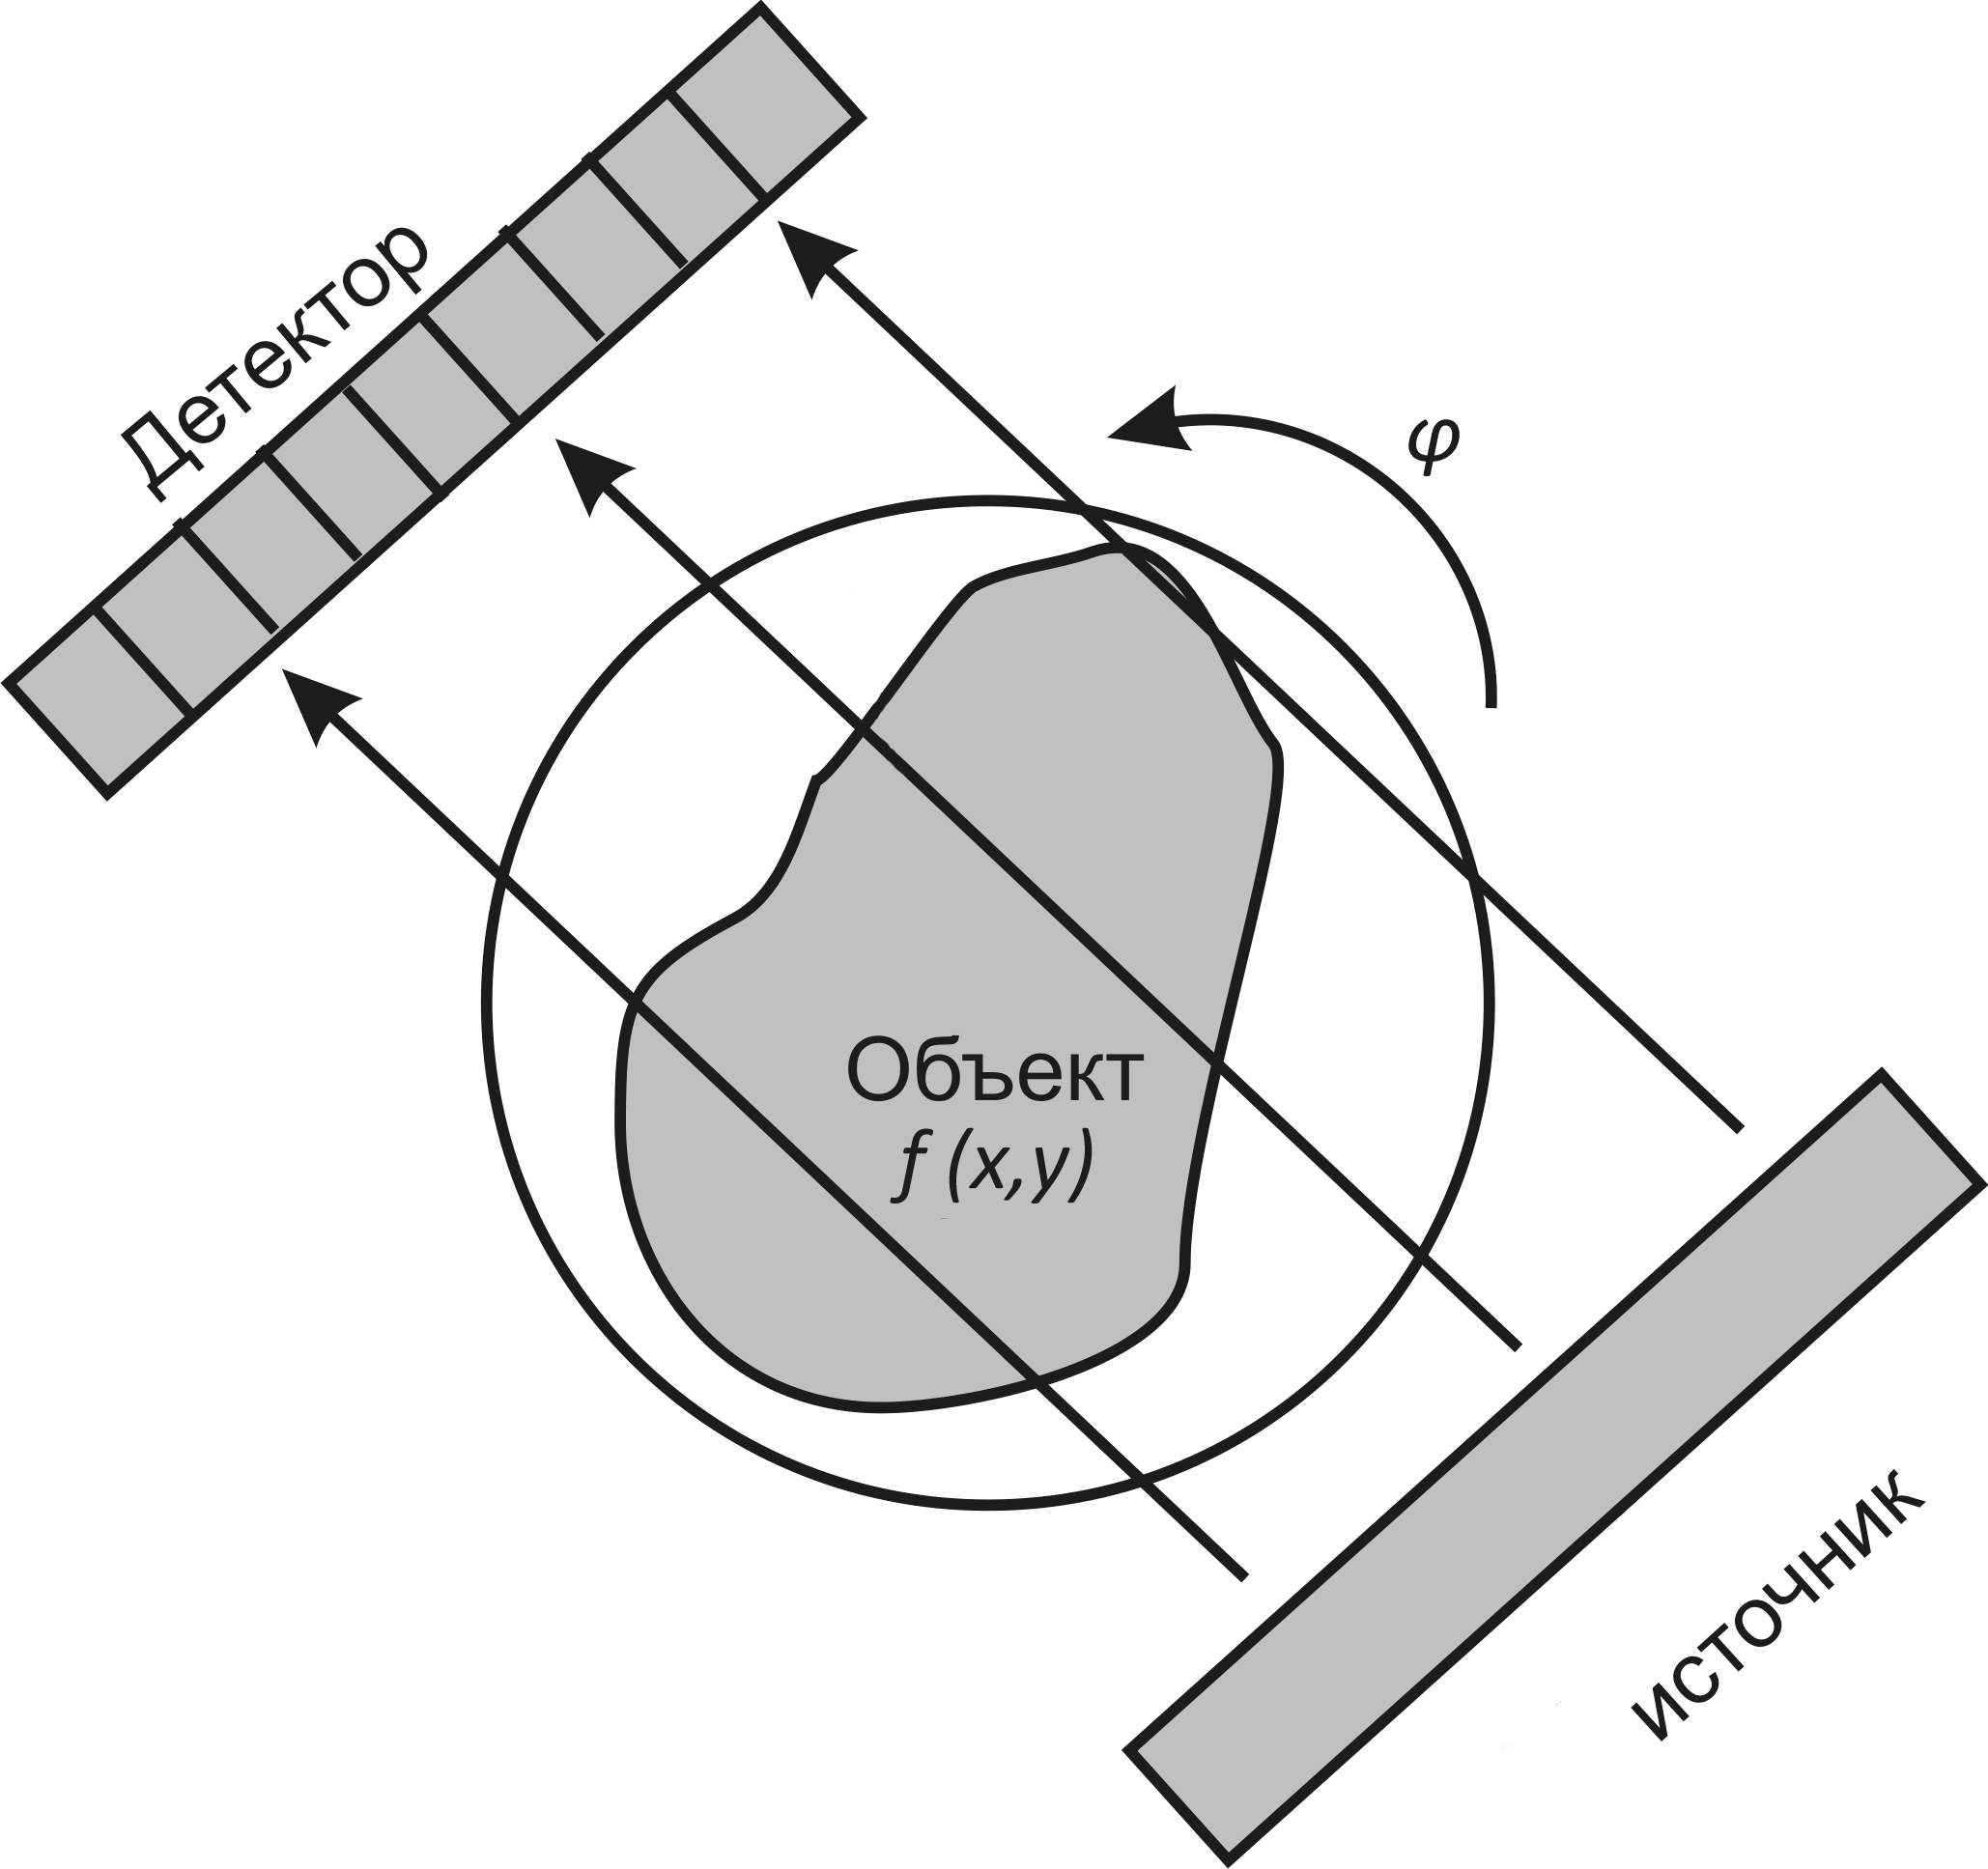
\includegraphics[width=0.45\textwidth]{../Dissertation/images/part1_img/experiment}
  \end{figure}
  &
  \begin{itemize}
  \item $N$ ячеек детектора
  \item $N_\varphi$ углов сканирования
  \item Для каждого угла $\varphi$ и каждой ячейки $\xi$ измеряется интенсивонсть прошедшего рентгеновского излучения \\
    $\mathrm I \left( \varphi, \xi \right) = \mathbb P (f(x, y))$ \\
    $\mathbb P$ --- оператор проекции \\
    $x, y$ --- координаты объекта

  \end{itemize}
\end{tabular}
\end{frame}

\begingroup
% \small

\begin{frame}
% \frametitle{Предмет исследования}
Компьютерная томография --- программно-аппаратный комплекс
% \pause
\setlength{\leftmargini}{0em}
\begin{columns}[T,onlytextwidth]
  \begin{column}{.4\textwidth}
  \begin{itemize}
    \item экспериментальная схема
    \item калибровка 
    \item \textbf{программная обработка $\rightarrow$}
  \end{itemize}
  \end{column}
  \pause
  \begin{column}[t]{0.4\linewidth}
  \begin{itemize}
    \item предобработка
    \item \textbf{алгоритмы восстановления $\rightarrow$}
    \item постобработка
  \end{itemize}
  \end{column}
  \pause
  \begin{column}[t]{0.35\linewidth}
  \begin{itemize}
    \item \textbf{метод оптимизации}
    \item \textbf{модель регуляризации}
    \item \textbf{физическая модель}
    \item реализация математических примитивов
  \end{itemize}
  \end{column}
\end{columns}
\end{frame}
\endgroup

% \begin{frame}
% \frametitle{План доклада}
% \begin{itemize}
% \item Подходы к решению задачи восстановления в КТ
% \item Алгоритм восстановления FHT-SIRT
% \item Учет наличия в объекте высокопоглощающих включений
% \item Метод восвзвешанных невязок
% \end{itemize}
% \end{frame}


\begin{frame}
\frametitle{Предположения}
\begin{itemize}
  \item Рассматривается плоское сечение
  \item Параллельная схема проекции
  \item Ослабление интенсивности излучения подчиняется закону Бугера:
\end{itemize}
  $$
  \mathrm I \left( \varphi, \xi , \lambda \right) = \mathrm I_0(\lambda) \exp\left( {-\int_{l(\varphi, \xi)} \! f(l, \lambda) \mathrm d l }\right),
  $$
  \small
  $f(x, y)$ ---  описывает распределение линейного коэффициента ослабления рентгеновского излучения \\
  $\mathrm I(\varphi, \xi, \lambda)$ --- зарегистрированная детектором интенсивность излучения длины волны $\lambda$ \\
  $\mathrm I_0(\lambda)$ --- интенсивность зондирующего излучения \\
  $l(\varphi, \xi)$ --- параметризация прямой под углом $\varphi$, и сдвигом $\xi$ \\
\end{frame}

\begin{frame}
\frametitle{Задача восстановления}
  Связь линейного коэффициента ослабления и интенсивности описывается преобразованием Радона $R[f(x,y)](\varphi, \xi)$:

  $$
  R[f](\varphi, \xi) = 
 \iint \! \mathrm d x \mathrm d y f(x,y)\delta(x\cos\varphi + y\sin\varphi - \xi)
  $$


  После логарифмирования закона ослабления:
  $$
  \ln \left (\frac{\mathrm I_0(\lambda)}{\mathrm I(\varphi, \xi, \lambda)} \right) = p(\varphi, \xi) = R[f](\varphi, \xi)
  $$

\end{frame}

\begin{frame}
\frametitle{Задача восстановления}
\begin{figure}
\centering
    прямая задача, модель измерения\\
    $\rightarrow$
    \\
    \begin{tabular}{p{0.1\textwidth} p{0.8\textwidth} p{01\textwidth}}
    \hspace{-1cm}
    \small{объект}
    &
    \hspace{-1cm} -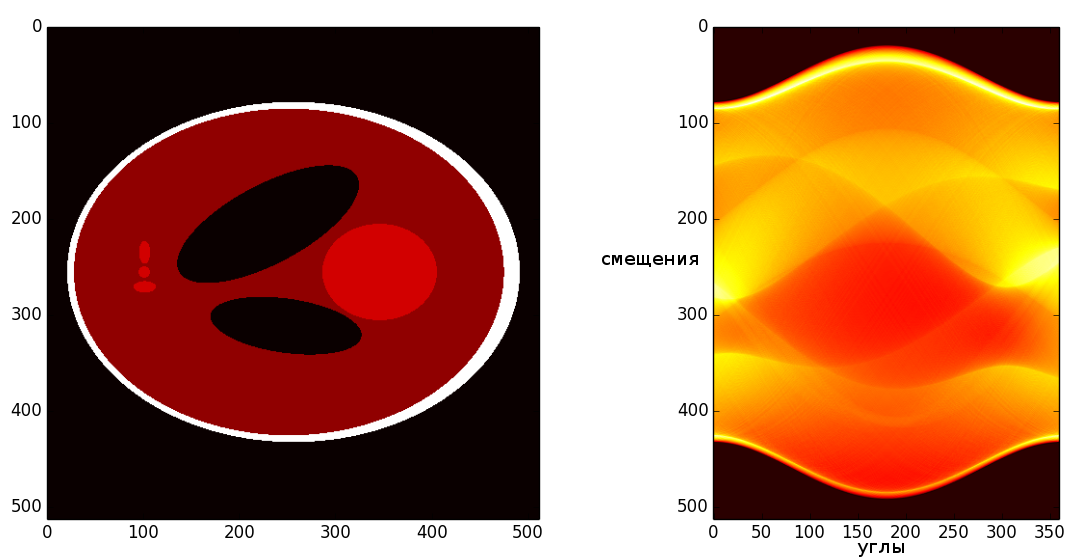
\includegraphics[width=0.8\textwidth]{sl_sinogram}
    &
    \hspace{-1cm} \small{измерения}
    \\
     \hspace{-1cm} \small{$f(x, y)$}
     &
    &
     \hspace{-1cm} \small{$p(\xi, \varphi)$}
    \end{tabular}
    \\
    $\leftarrow$ \\
    обратная задача, процедура восстановления
\end{figure}
\end{frame}

% \begin{frame}
% \frametitle{Задача восстановления}
% 
% Задача восстановления функции $f(x,y)$- задача обращения преобразования Радона полученных измерений $p$:
% $$
% f(x,y) = R^{-1}(p(\varphi, \xi))
% $$
% \end{frame}


\section{Подходы к решению задачи восстановления в КТ}
\begingroup
\small
\begin{frame}
\frametitle{Методы восстановления}
\begin{tabular}{p{0.15\textwidth} | p{0.4\textwidth} | p{0.4\textwidth}}
\hspace{-1cm} семейство & Интегральные & Алгебраические \\ \hline \vspace{10pt}
\hspace{-1cm} подход & формула для обращения $R^{-1}[p(\varphi, \xi)](x,y)$ & Оптимизационная задача $\min_{f} \Norm{R[f] - p}$\\ \hline \vspace{5pt}
\hspace{-1cm} представители & \footnotesize{Filtered Backprojection (FBP)} & \footnotesize{Algebraic Reconstruction Technique (ART),\ Simultaneous ART (SART),\ Simultaneous Iterative RT (SIRT) }\\ \hline \vspace{3pt}
\hspace{-1cm} сложность & $O(N^2 \log N)$ & $O(N^3)$ \\ \hline \vspace{5pt}
\hspace{-1cm} особенности & универсальность & возможность учета модели объекта или \\
                          & требует полного набора проекционных углов, их равномерного распределения  & измерительной схемы \\ 
                          & чувствительны к шумам & \\
\end{tabular}
\\
\vspace{3pt}
$N$ --- число ячеек детектора
\end{frame}
\endgroup

\begin{frame}
\frametitle{Метод Свертки и обратной проекции}
\begin{columns}
  \hspace{-0.1cm}
  \begin{column}{0.6\textwidth}
    Основные шаги метода:
    \begin{itemize}
    \item Фильтрация проекций: $\tilde{p}(\xi, \varphi) = \mathscr F ^{-1}[|u| \mathscr F[p(\xi, \varphi)](u)]$\\
    $\mathscr F[\cdot], \mathscr F ^{-1}[\cdot]$ --- прямое и обратное преобразования Фурье по $\xi$\\
    \vspace{10pt}
    \item Вычисление обратной проекции $f(x,y) = \int_0^\pi {\tilde{p} (x \cos\varphi + y \sin \varphi, \varphi) d\varphi}$
    \end{itemize}
  \end{column}

  \begin{column}{0.6\textwidth}
  Достоинства:
  \begin{itemize}
    \item скорость работы
    \item универсальность
    \item точная формула (при непрерывных значениях $\xi, \varphi$)
  \end{itemize}
  Недостатки:
  \begin{itemize}
    \item требует равномерную сетку углов
    \item чувствителен к шумам
    \item не позволяет учитывать специфики эксперимента
  \end{itemize}
  \end{column}
\end{columns}
\end{frame}

\begin{frame}
\centering
\frametitle{Метод Свертки и обратной проекции}
  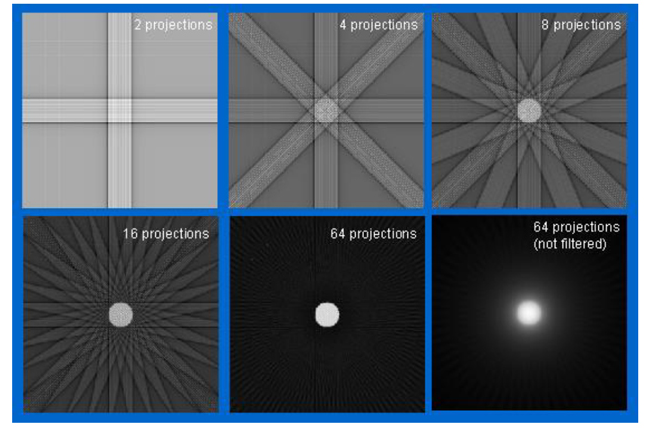
\includegraphics[width=0.8\textwidth]{fbp_img.png}
  \\
  Операция обратной проекции
\end{frame}

%\section{Вычислительно эффективный алгебраический метод восстановления FHT-SIRT}

\begin{frame}
\frametitle{Алгебраический метод}
\framesubtitle{Основные положения}
\begin{itemize}
  \item непрерывные функции $\rightarrow$ дискретные изображения:

    {
    \centering
    $f(x,y) \rightarrow f_i,\ p(\varphi, s) \rightarrow p_j$
    \par
    }
  \vspace{0.5cm}
  \item преобразование Радона $\rightarrow$ преобразование Хафа:
  
    {
    \centering
    $R[f](\varphi, s) \rightarrow (\mathrm W f)_j$ 
    \par
    }
  \vspace{0.5cm}

    $\mathrm W$ --- матрица проекции, указывает вклад пикселя $i$ в лучевую сумму вдоль луча $j$.\\
    Разреженная матрица размера $N_\varphi * N^3$, в которой только порядка $O(N_\varphi * N^2)$ ненулевых элементов
    \vspace{0.5cm}
  \item решение разреженной СЛАУ большой размерности итерационным методом

    {
    \centering
    $p = \mathrm W f$
    \par
    }

\end{itemize}
\end{frame}

\begin{frame}
\frametitle{Матрица проекции W}
\begin{tabular}{c c c}
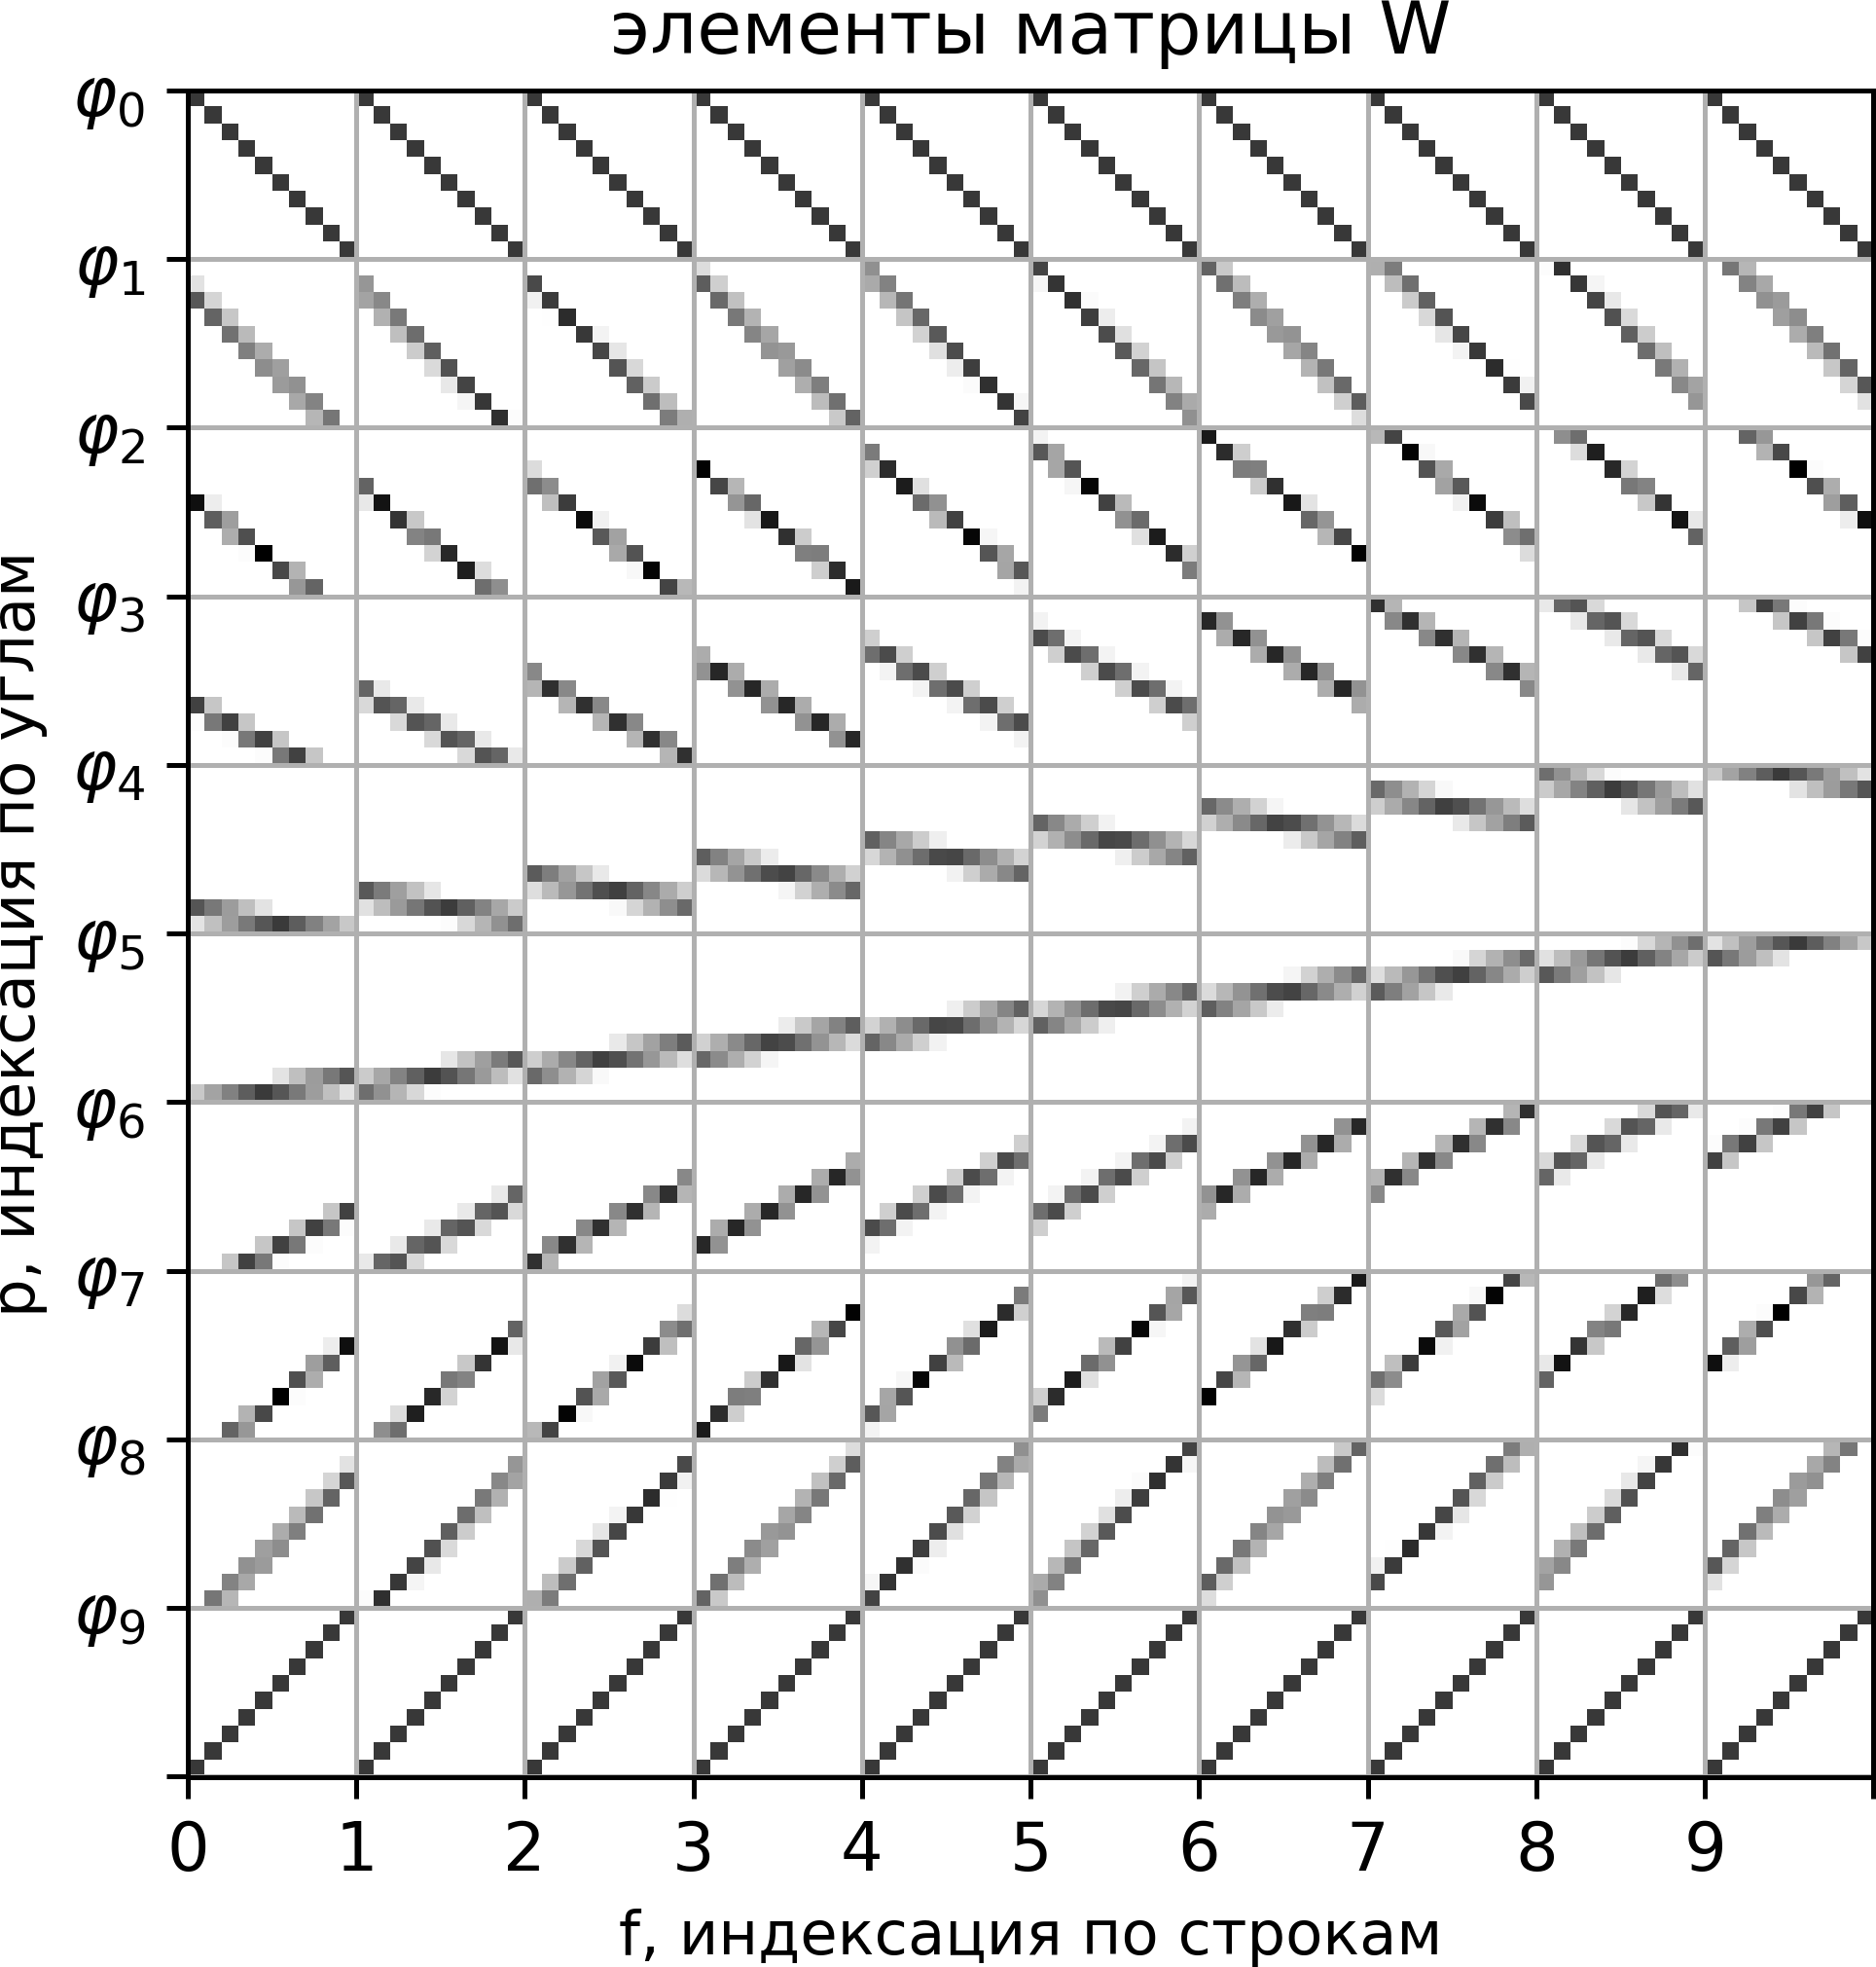
\includegraphics[width=0.4\textwidth]{w_matrices/W_10_10_plot.png} &
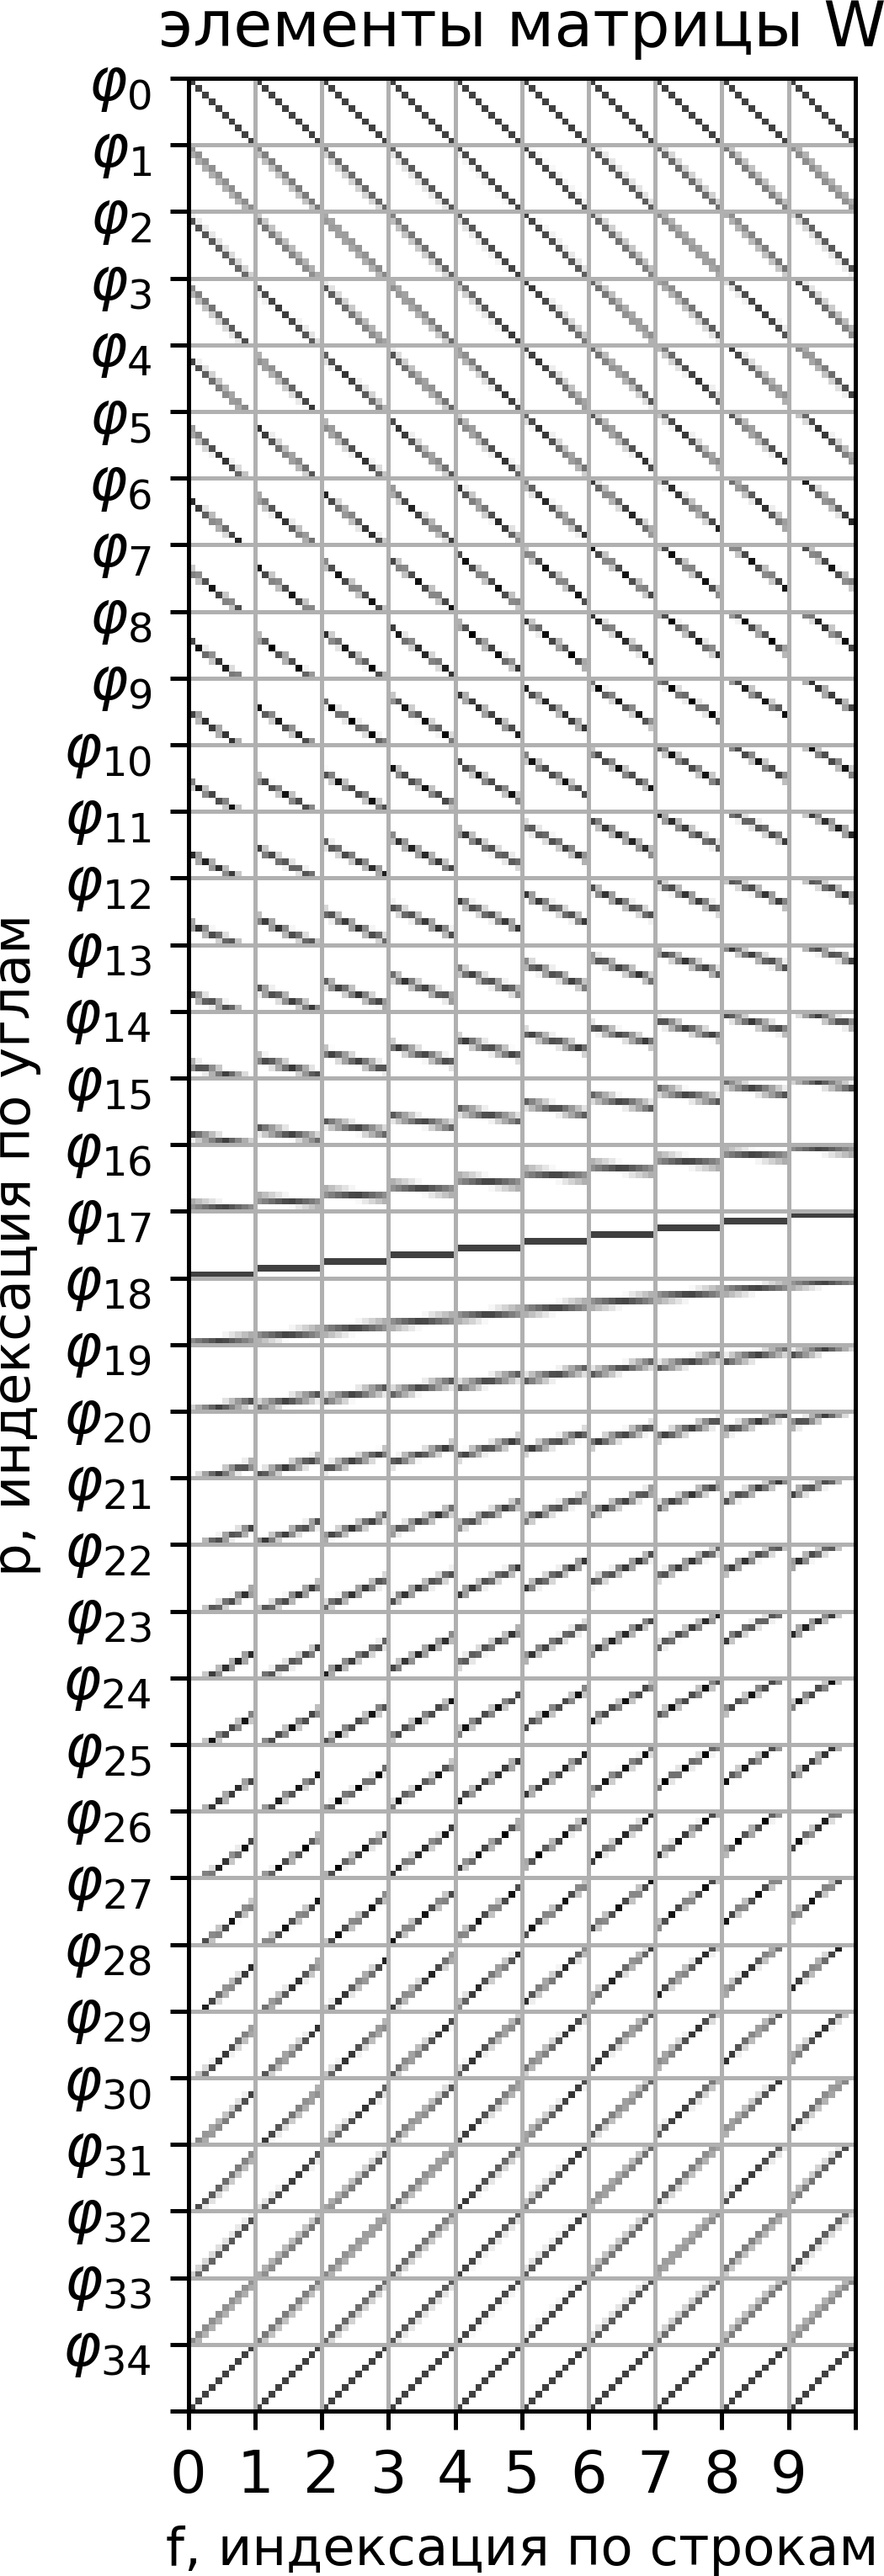
\includegraphics[height=0.8\textheight]{w_matrices/W_10_35_plot.png} &
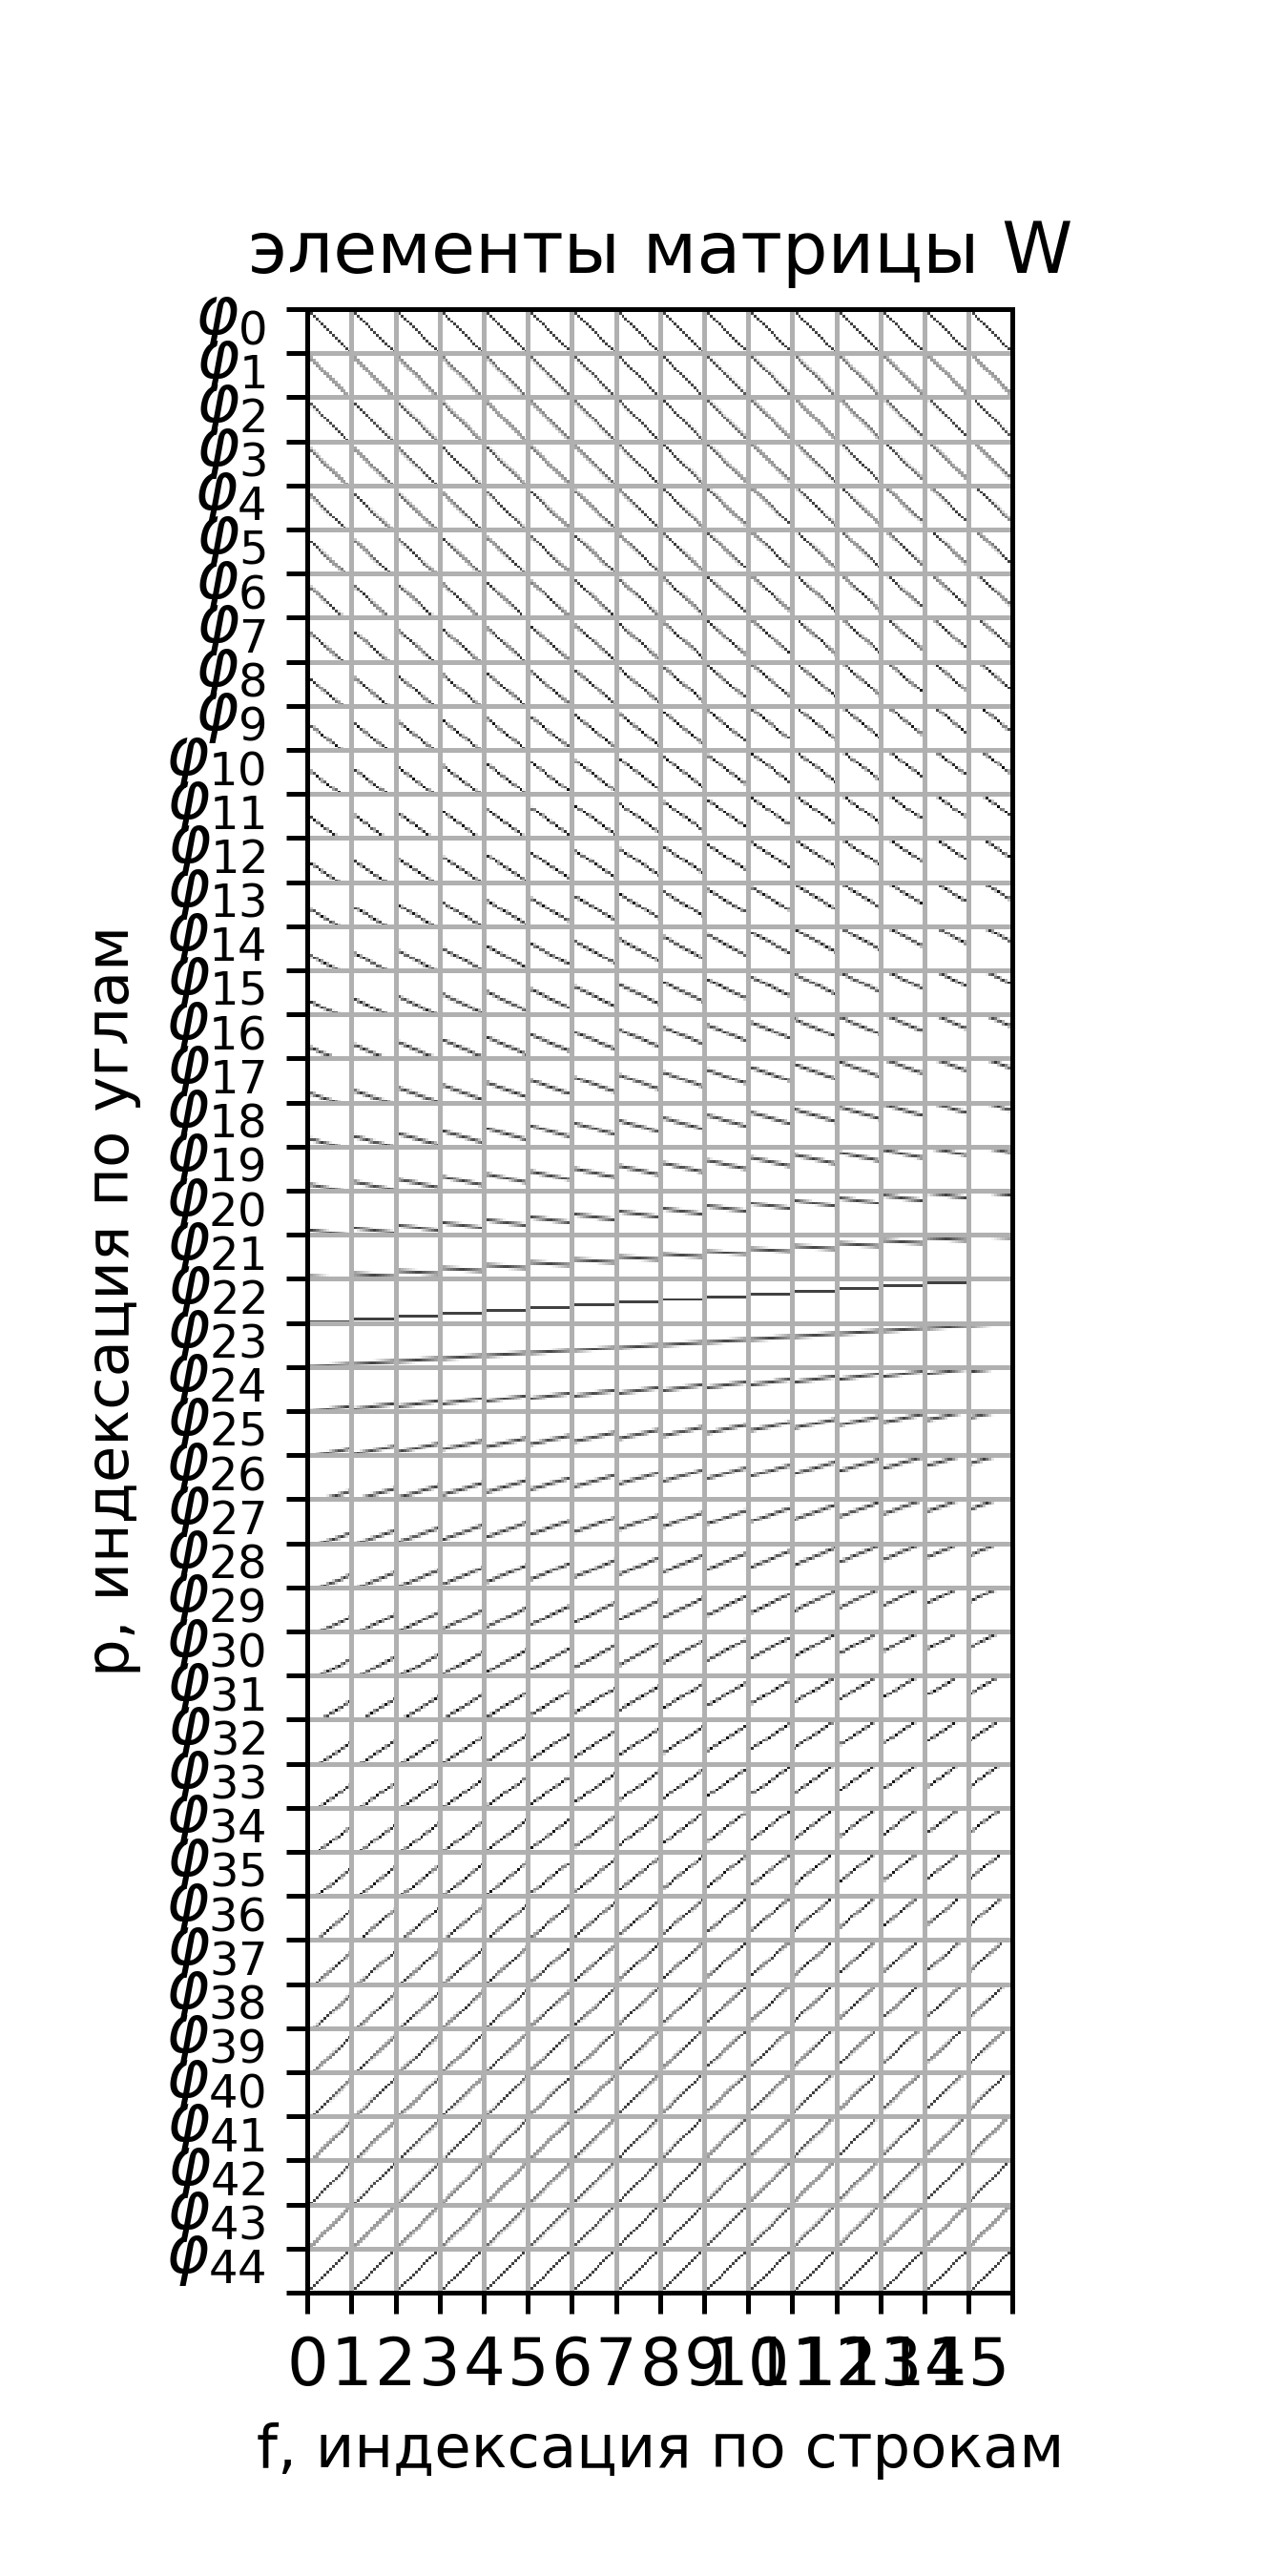
\includegraphics[height=0.8\textheight]{w_matrices/W_16_45_plot.png} \\
\small{$N = 10$, $N_\varphi = 10$} &
\small{$N = 10$, $N_\varphi = 35$} & 
\small{$N = 16$, $N_\varphi = 45$}
\end{tabular}
\end{frame}

\begin{frame}
\frametitle{Алгебраический метод}
\framesubtitle{Решение СЛАУ}
\centering
$\Norm{p - \mathrm W f} \rightarrow \min\limits_f$

Оптимизационная задача решается итерационным методом, шаг итерации имеет вид
\vspace{0.5cm}

\begingroup
\footnotesize

\hspace*{-0.5cm}
\begin{tabular}{c|c|c}
ART & SART & SIRT \\ \hline
для каждого луча & для каждого угла & для всех лучей\\
$j = 1 \dots N * N_\varphi$ & $\varphi_k$ & \\
$\hat{f} = f - \gamma \mathrm W^{\mathrm T}_j(\mathrm W f - p)$ &
$\hat{f} = f - \gamma \mathrm {W^{\varphi_k}}^{\mathrm T}(\mathrm W f - p)$ &
$\hat{f} = f - \gamma \mathrm W^{\mathrm T}(\mathrm W f - p)$ \\
\end{tabular}

\vspace{0.2cm}
\raggedright
\endgroup

$\mathrm W_j$ --- столбец матрицы для луча $j$,\\
$\mathrm W^\varphi$ ---  матрица проекции на угол $\varphi$, $\mathrm W = \sum_\varphi {\mathrm W^\varphi}$
\\
\vspace{0.4cm}

$\mathrm W f$ --- прямая проекция, \\
$\mathrm W^{\mathrm T} f$ --- обратная проекция.
\end{frame}


\begin{frame}
\frametitle{SIRT}
\framesubtitle{Анимация процесса восстановления}
\begin{columns}[T,onlytextwidth]
\begin{column}{0.4\textwidth}
\animategraphics[loop,controls,width=\linewidth]{10}{anim/frame_}{1}{60}
\end{column}

\begin{column}{0.6\textwidth}
\animategraphics[loop,controls,width=\linewidth]{10}{anim/slice_}{1}{60}
\end{column}
\end{columns}
%\endgroup
\end{frame}

\begin{frame}
\frametitle{Алгебраический метод}

Преимущества:\\
\begin{itemize}
  \item качество восстановления
  \item возможность учета специфики эксперимента (регуляризация, ограничения)
\end{itemize}
\vspace{1.5cm}

Недостатки:\\
\begin{itemize}
  \item сложность настройки
  \item низкая скорость работы
  \item сходимость
\end{itemize}
\end{frame}

\begin{frame}
\frametitle{Направления развития алгебраических методов}

\begin{itemize}
  \item \textbf{ускорение}
  \begin{itemize}
    \item использование GPU
    \item \textbf{улучшение асимптотики итерации}
    \item ускорение сходимости итерационной процедуры
  \end{itemize}
  \item \textbf{улушчение качества восстановления, борьба с артефактами}
    \begin{itemize}
    \item огрубление луче (beam hardening)
    \item \textbf{артефакты из-за сильнопоглощающих включений (metal artifacts)}
    \end{itemize}
  \item \textbf{учет спектра источника} \\
  \small{В условиях лабороторного спектра восстановленная характеристика является усреднением линейного коэффициента полгощения по спектру. Это затрудняет интерпретацию результатов восстановления. }
\end{itemize}

\end{frame}

\section{Вычислительно эффективный алгебраический метод восстановления FHT-SIRT}
% \section{Вычислительно эффективный алгебраический метод восстановления FHT-SIRT}

\begin{frame}
\frametitle{FHT-SIRT: основная идея}
\centering
\begin{columns}
\begin{column}{0.35\textwidth}
\centering
FBP\\
\vspace{20pt}
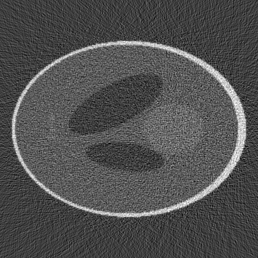
\includegraphics[width=1\textwidth]{sl_fbp_noisy}\\
\vspace{20pt}
$O(N^2 \log N)$
\end{column}
\vrule{}
\begin{column}{0.35\textwidth}
\centering
SIRT\\
\vspace{20pt}

\includegraphics[width=1\textwidth]{sl_art_good}\\
\vspace{20pt}
$O(N^3)$
\end{column}
\vrule{}
\begin{column}{0.35\textwidth}
\centering
FHT-SIRT\\
\vspace{20pt}

\includegraphics[width=1\textwidth]{sl_art_good}\\
\vspace{20pt}
$O(N^2 \log N)$
\end{column}
\end{columns}
\end{frame}

\begin{frame}
\frametitle{Быстрое преобразование Хафа}
\framesubtitle{БПХ, FHT}
\begin{columns}[T,onlytextwidth]
  \hspace*{-0.5cm}
  \begin{column}{0.65\textwidth}
  Приближенный способ вычисления сумм интенсивностей изображения вдоль всевозможных прямых
  \begin{figure}
    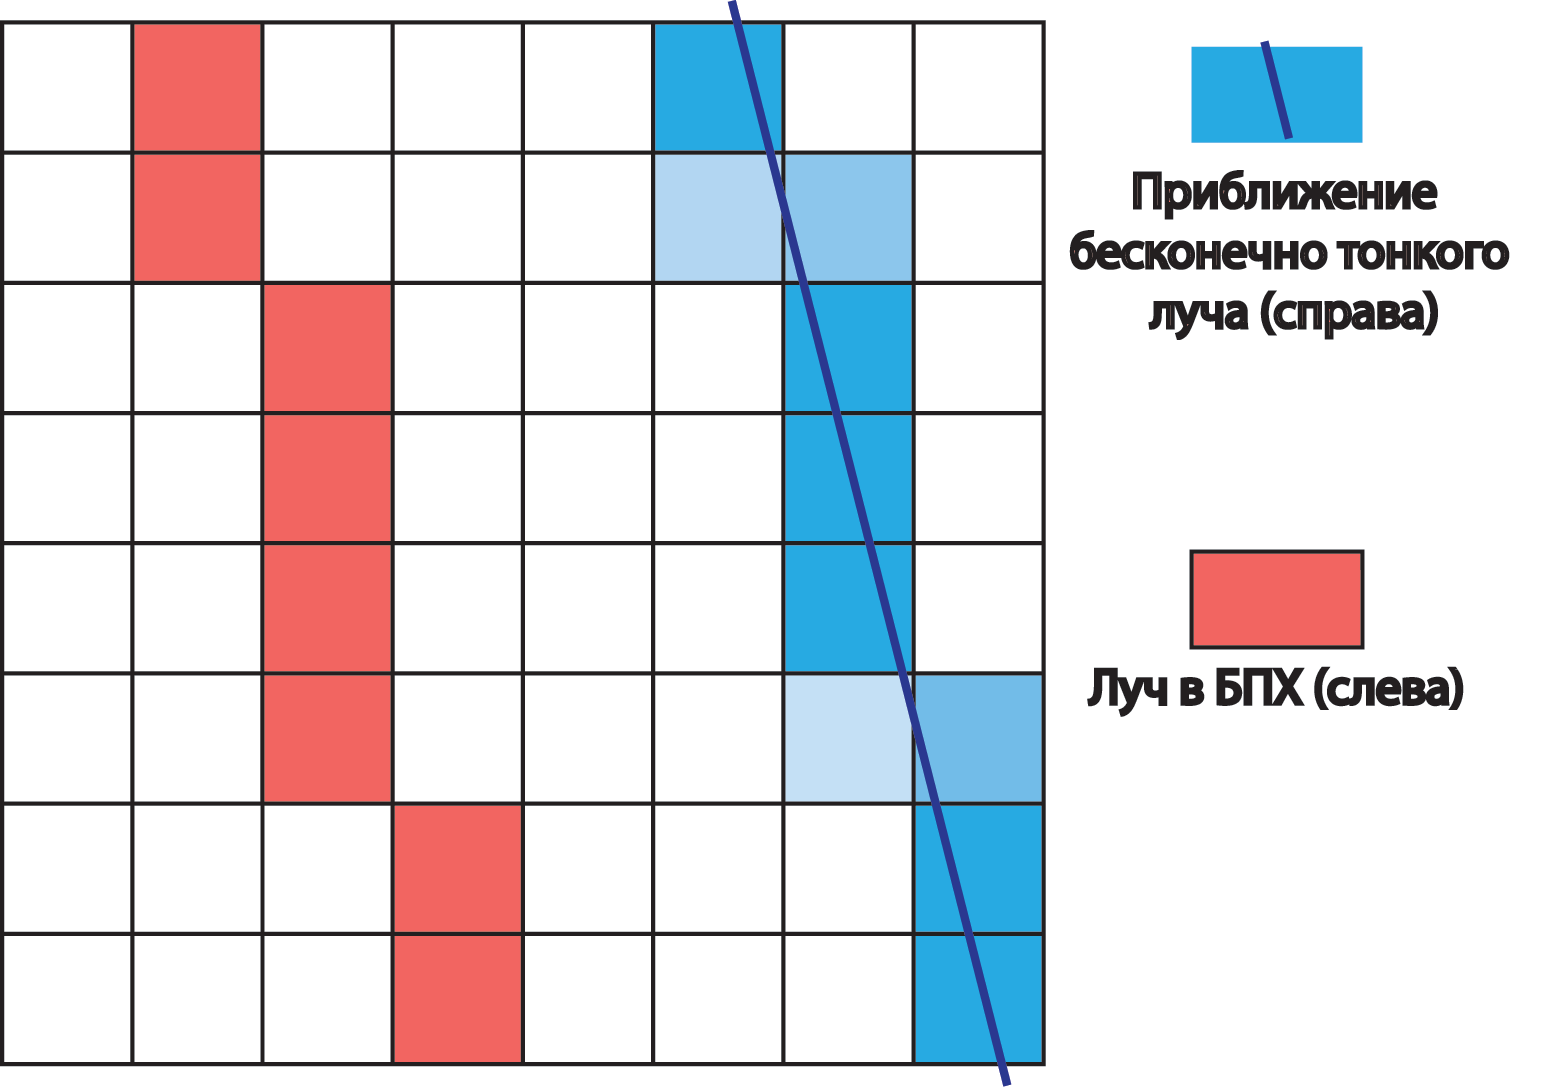
\includegraphics[width=1\textwidth]{fht}
  \end{figure}
  \end{column}
  \begin{column}{0.45\textwidth}
  \begin{itemize}
    \item диадические паттерны суммирования
    \item рекурсивная процедура построения
    \item для больших размеров изображения хорошо приближает прямые (отклонение не превышает  $\frac 1 6 \log N$ ) %\cite{ershov2015dyadic})
    \item асимптотическая сложность $O(N^2 \log N)$
  \end{itemize}
  \end{column}
\end{columns}

\end{frame}

\begin{frame}
\frametitle{Процедура формирования паттернов}
  \begin{figure}
  \centering
    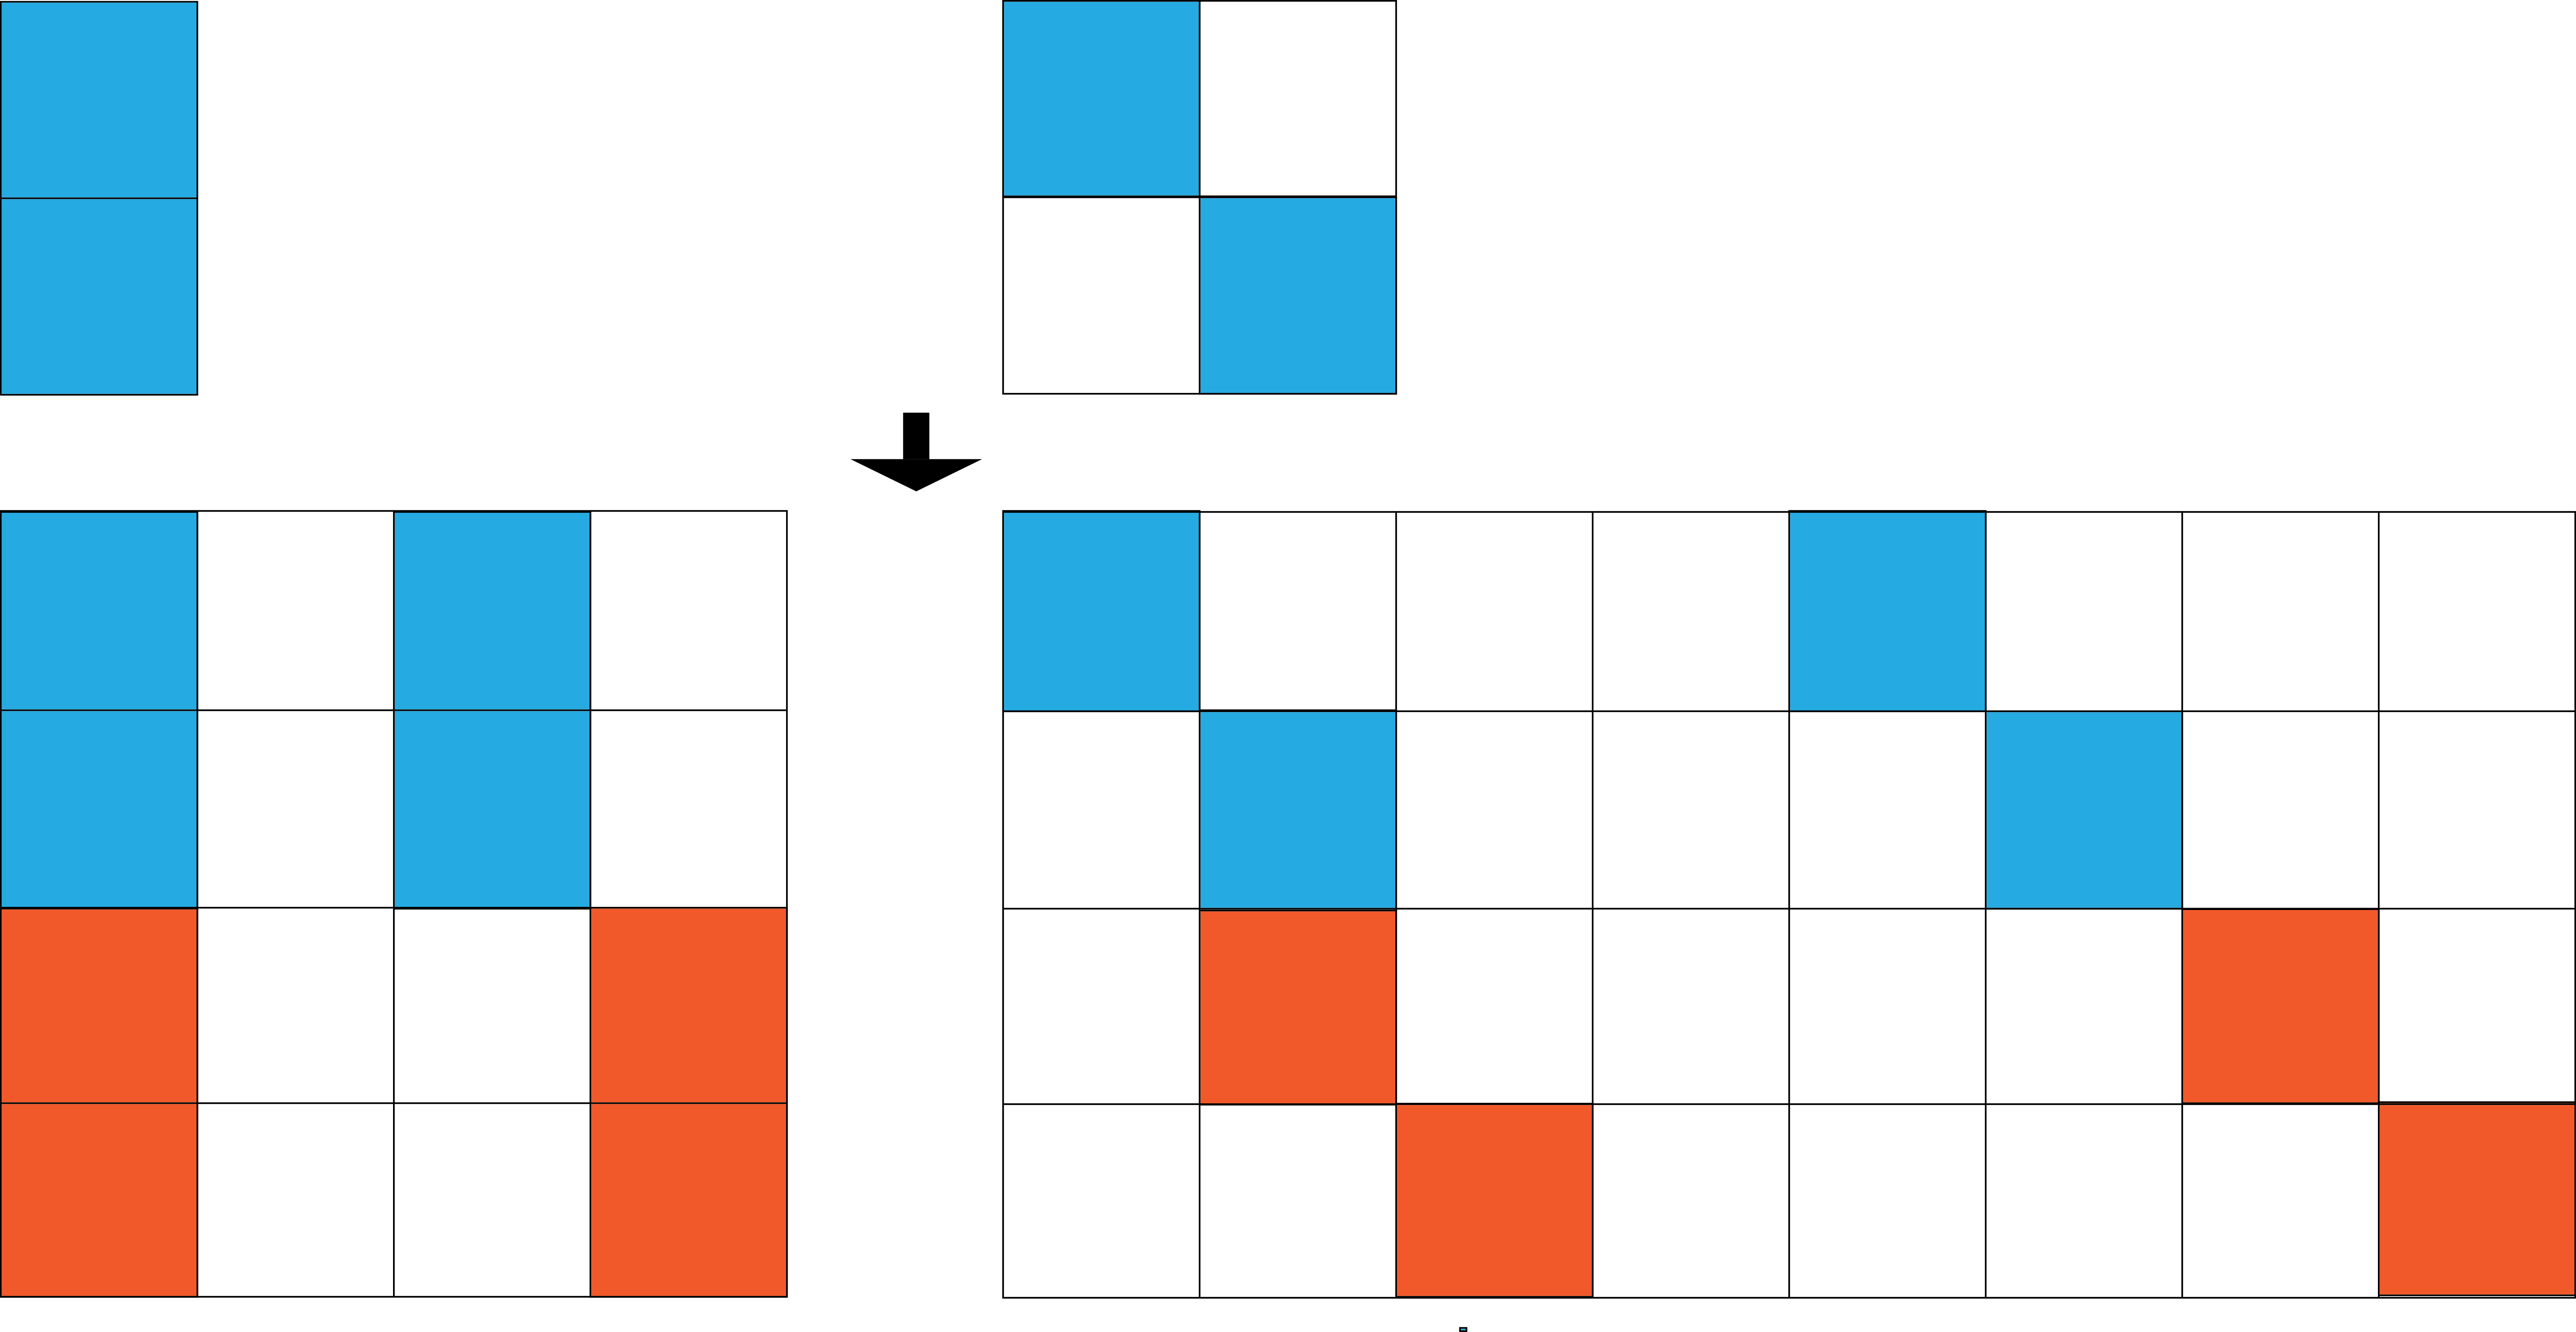
\includegraphics[width=1\textwidth]{../Dissertation/images/part1_img/hough_proc}
  \end{figure}
\end{frame}

\begin{frame}
\frametitle{Быстрое преобразование Хафа}
\framesubtitle{вид матрицы W}
\centering
\begin{columns}

\column{0.2\textwidth}
Обычная проекция \\
$N = 10$ \\
$N_\varphi = 35$

\column{0.3\textwidth}
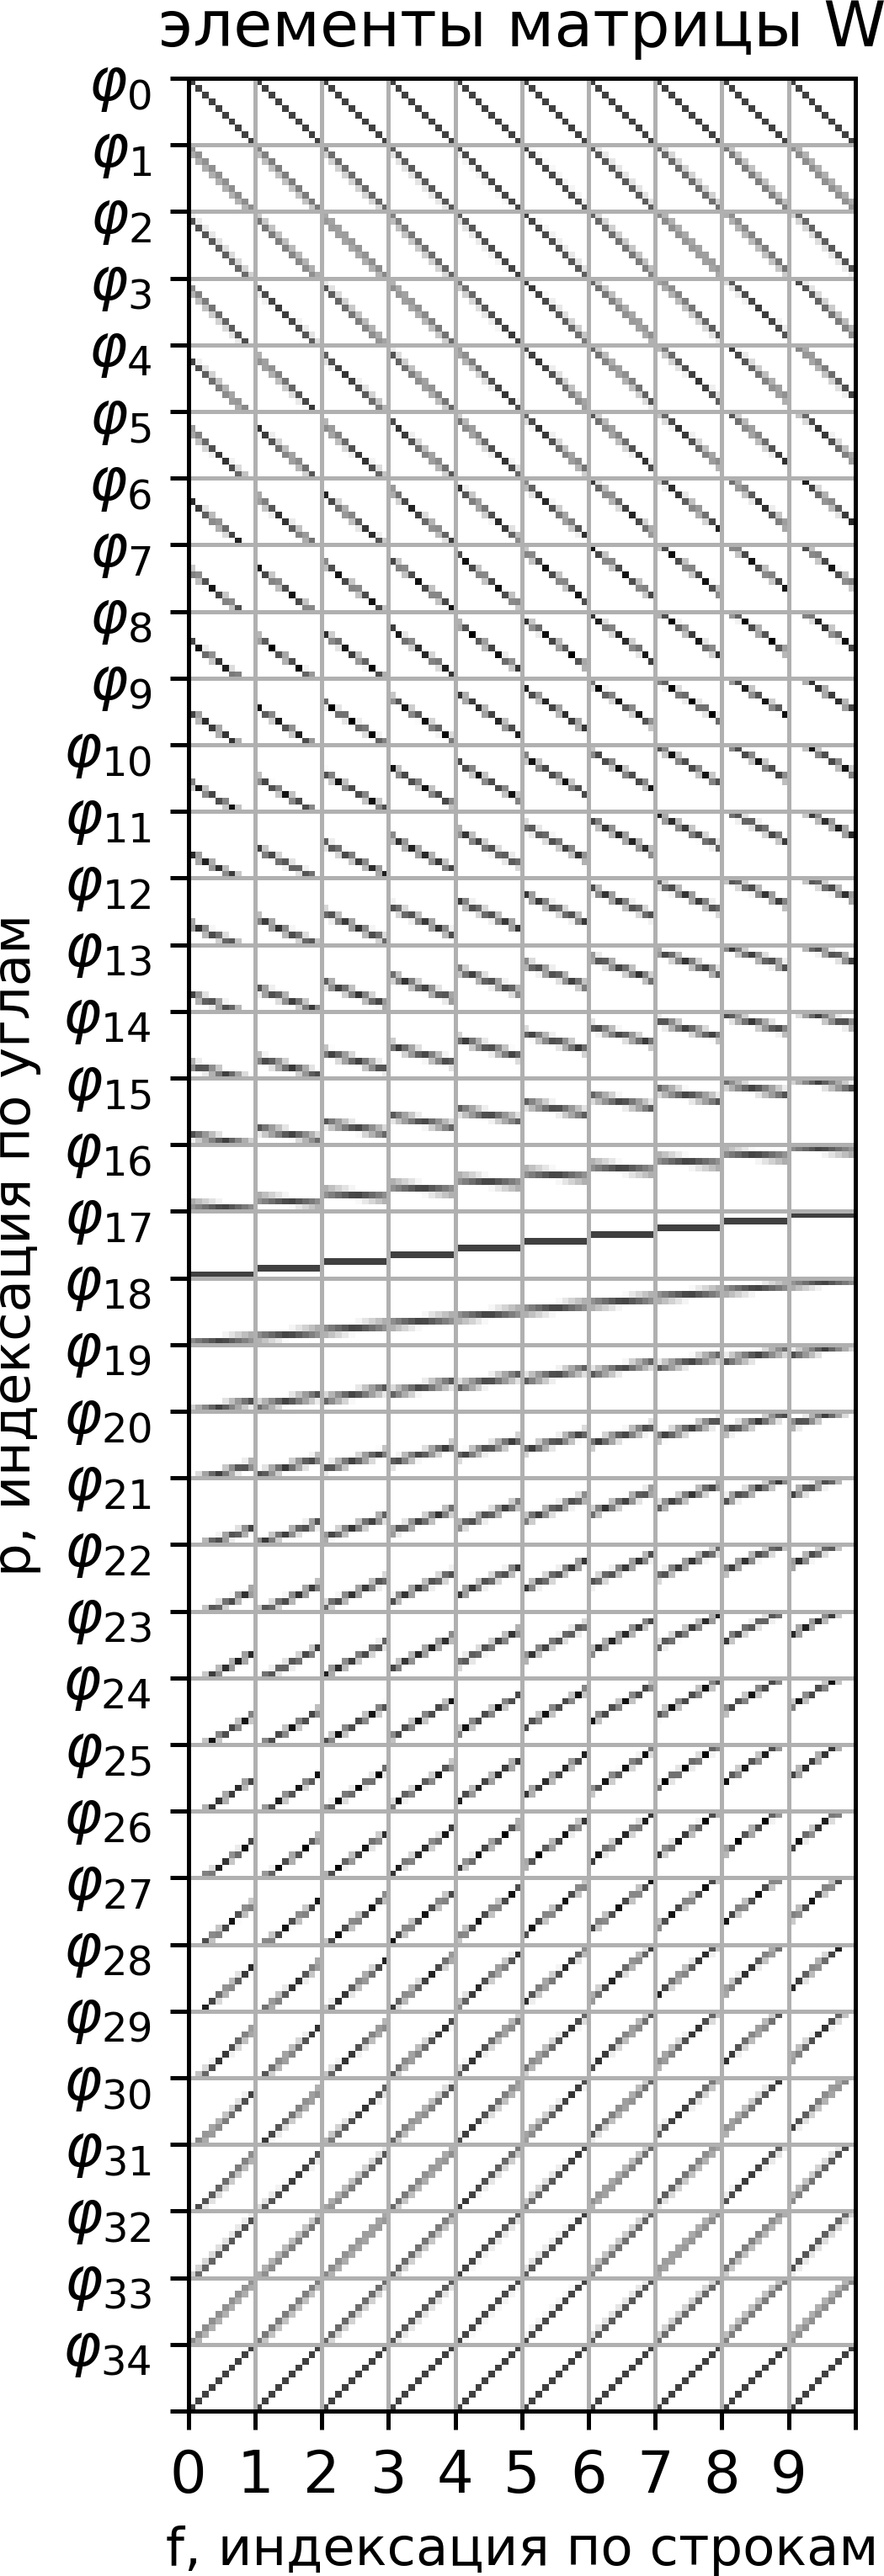
\includegraphics[height=0.7\textheight]{w_matrices/W_10_35_plot.png}

\column{0.3\textwidth}
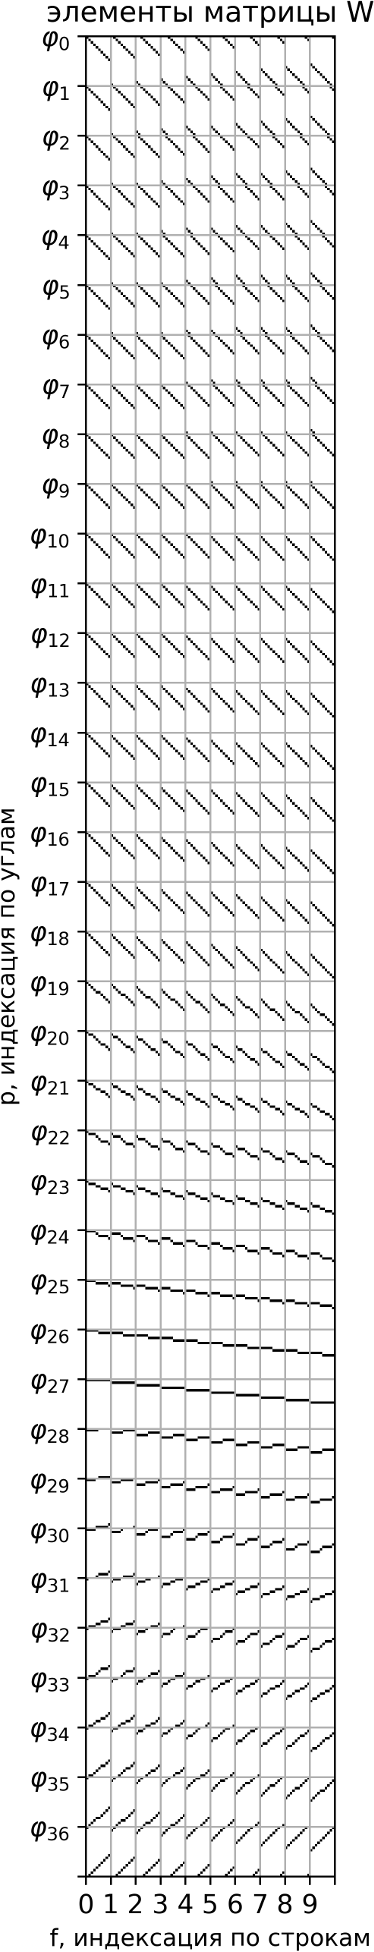
\includegraphics[height=0.80\textheight]{w_matrices/W_FHT_10_plot.png}

\column{0.2\textwidth}
БПХ \\
$N = 10$ \\
$N_\varphi = 37$ \\
\end{columns}
\end{frame}

\begin{frame}
\frametitle{Быстрое преобразование Хафа}
\framesubtitle{вид матрицы W}
\centering
\begin{columns}

\column{0.2\textwidth}
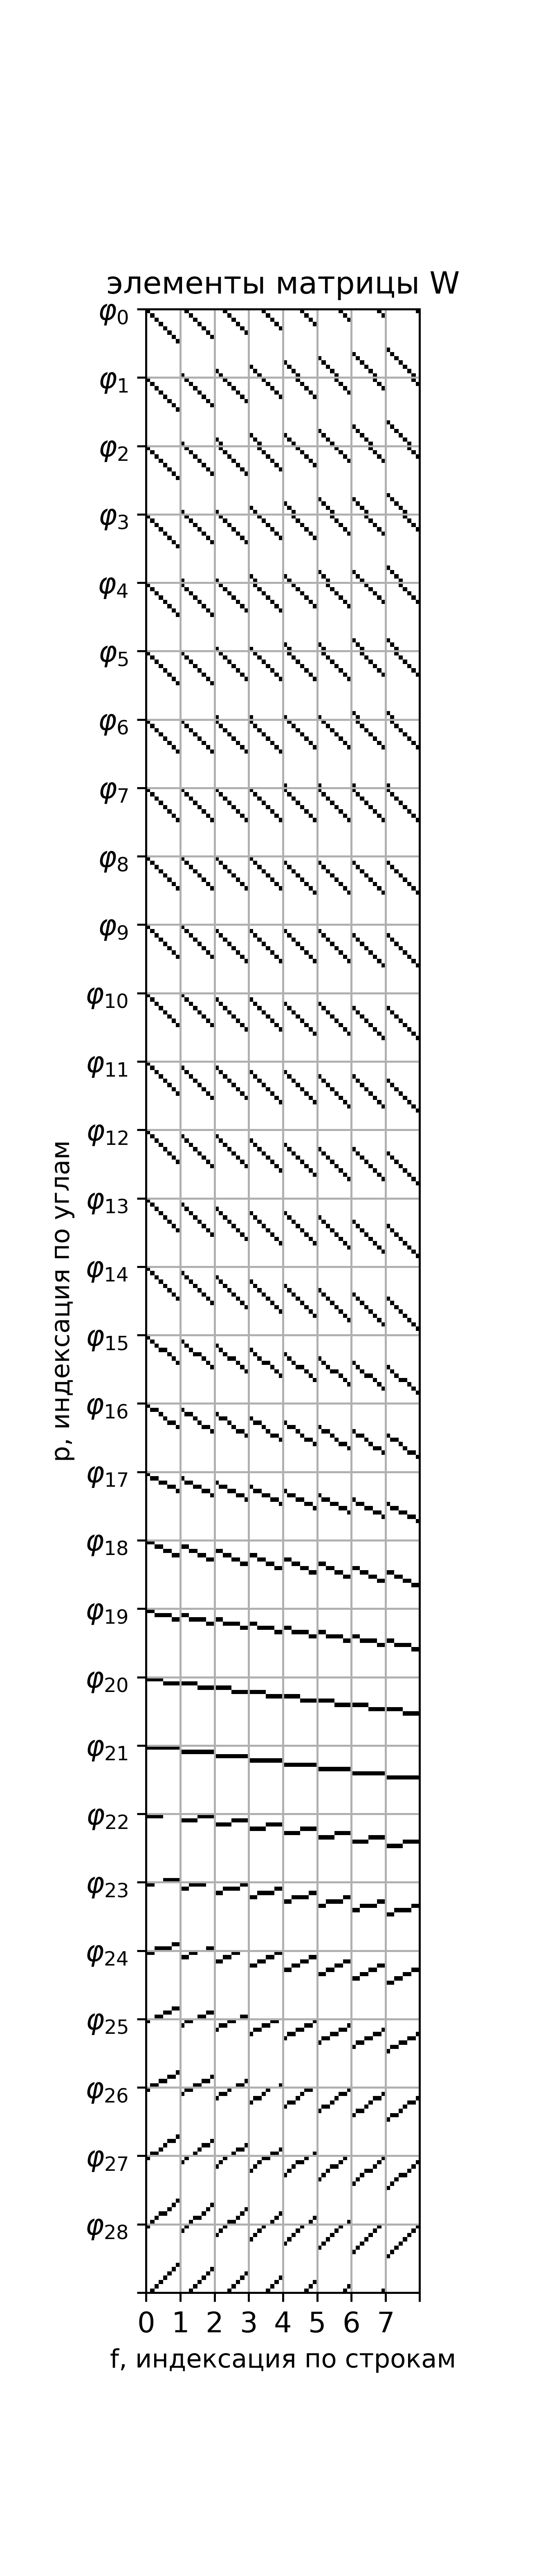
\includegraphics[height=0.9\textheight]{w_matrices/W_FHT_8_plot.png}

\column{0.2\textwidth}
$N = 8$ \\
$N_\varphi = 29$

\column{0.1\textwidth}

\includegraphics[height=0.9\textheight]{w_matrices/W_FHT_16_plot.png}

\column{0.2\textwidth}
$N = 16$ \\
$N_\varphi = 61$


\column{0.1\textwidth}
\includegraphics[height=0.9\textheight]{w_matrices/W_FHT_32_plot.png}

\column{0.2\textwidth}
$N = 32$ \\
$N_\varphi = 125$ \\

\end{columns}

\end{frame}

\begin{frame}
\frametitle{FHT-SIRT}
\framesubtitle{прямая проекция}
\begin{columns}[T,onlytextwidth]
  \hspace*{-0.5cm}
  \begin{column}{0.65\textwidth}
  \begin{figure}
    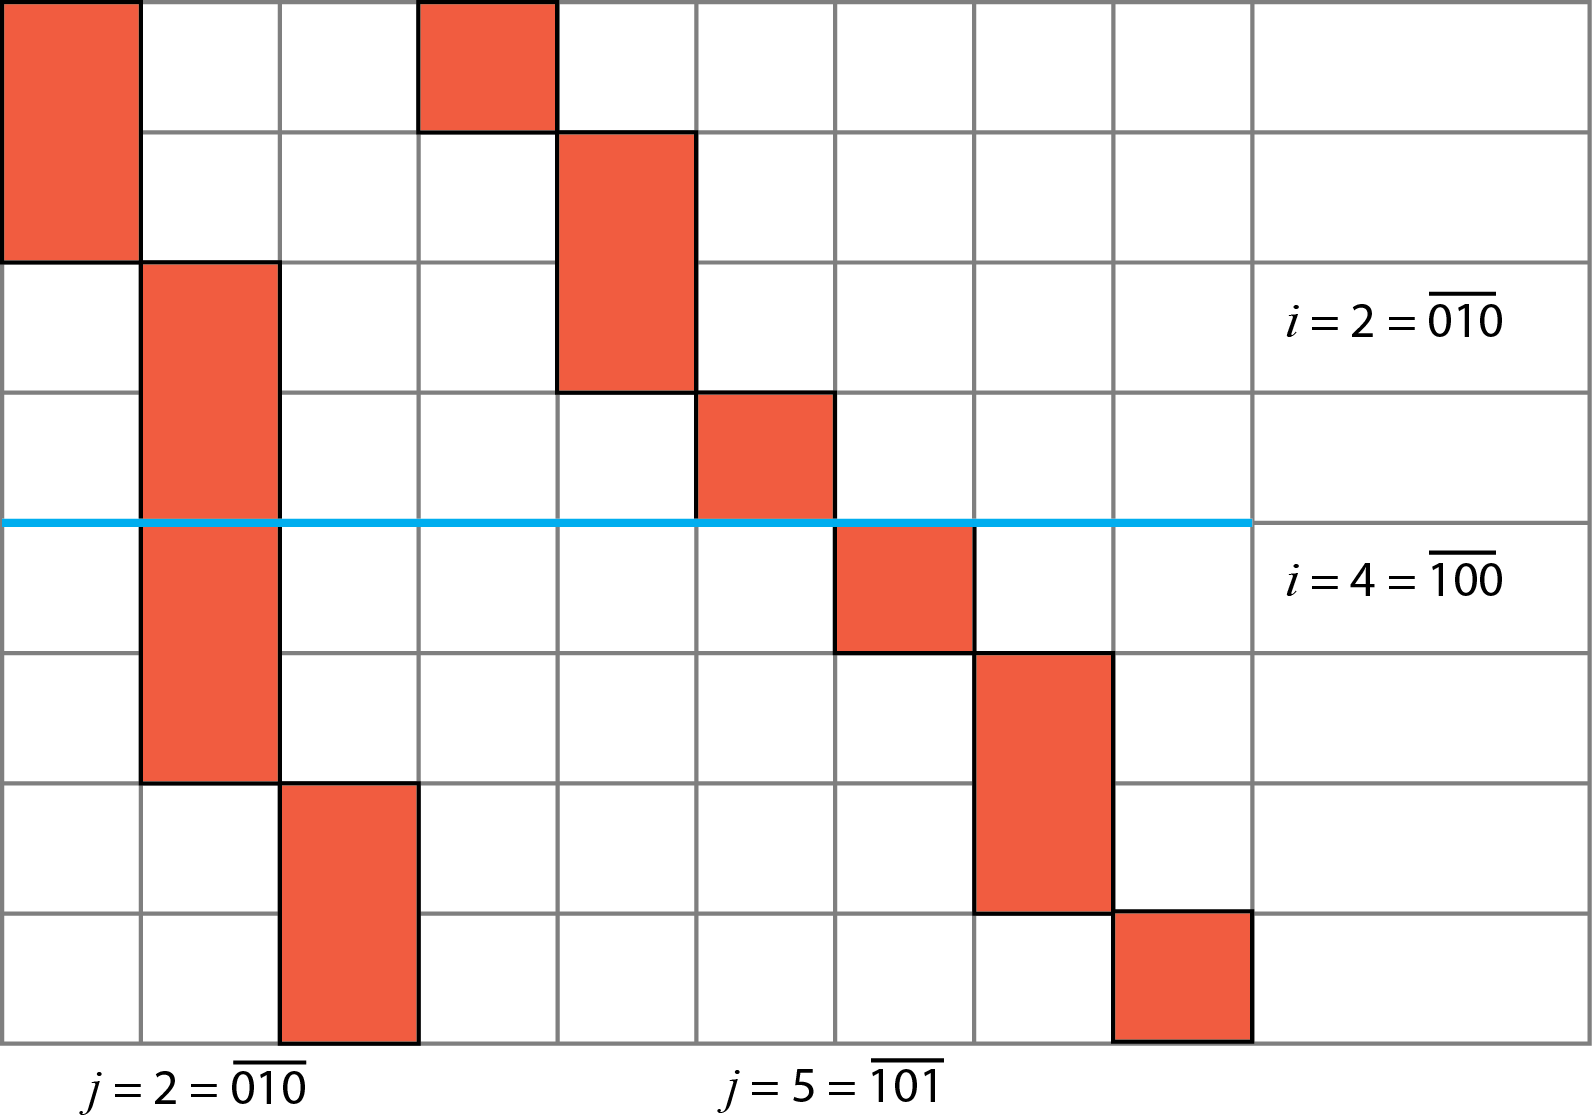
\includegraphics[width=\textwidth]{../Dissertation/images/part1_img/pattern_structure}
  \end{figure}
  \end{column}
  \begin{column}{0.45\textwidth}
    Углы в БПХ делятся на 4 группы:
    \begin{equation} \notag
    \begin{array}{lll}
    \alpha^\rom{1}_i &= \pi - & \arctan{\frac{N-1-i}{N-1}} \\
    \alpha^\rom{2}_i &= &\arctan{\frac{i - (N-1)}{N-1}} \\
    \alpha^\rom{3}_i &= \frac \pi 2 - & \arctan{\frac{3(N-1)-i}{N-1}} \\
    \alpha^\rom{4}_i &= \frac \pi 2 - & \arctan{\frac{i - 3(N-1)}{N-1}}
    \end{array}
    \end{equation}

    Вычисление прямой проекции в шаге FHT-SIRT имеет вид 
        $\mathrm W = \left( \mathrm  W^\rom{1}\ \mathrm W^\rom{2}\ \mathrm  W^\rom{3}\ \mathrm  W^\rom{4} \right)^{\mathrm T}$.
  \end{column}
\end{columns}
\end{frame}


\begin{frame}
\frametitle{FHT-SIRT}
\framesubtitle{обратная проекция}

\begingroup
\small
\vspace{-0.5cm}
\newtheorem{myth}{Лемма}\
\begin{myth}
Пусть $pattern_j$ --- вертикальный паттерн скоса для j'ой строки преобразования Хафа изображения высотой $M_s = 2^n$.
Тогда имеет место равенство:
\begin{equation} \notag
\label{statement1}
\begin{array}{l l}
pattern_j[i] = pattern_i[j] & \quad  i,j \in \overline{1, 2^n},
\end{array}
\end{equation}
т. е. матрица, составленная из паттернов скоса, записанных в качестве столбцов, симметрична.
\end{myth}
\endgroup
\noindent\rule{8cm}{0.4pt}
\vspace{0.3cm}

Откуда следует, что ${W^{\mathrm K}} ^ {\mathrm T} = W^{\mathrm K}$, а значит
$$
W^{\mathrm T} q = \sum_{K=\rom{1}}^{K=\rom{4}}{W^{\mathrm K} q}
$$

\end{frame}


\begin{frame}
\frametitle{FHT-SIRT}
\framesubtitle{исследование работы}

\begin{columns}[T,onlytextwidth]
  \hspace*{-0.5cm}
  \begin{column}{0.53\textwidth}
    \begin{figure}
      \centering
      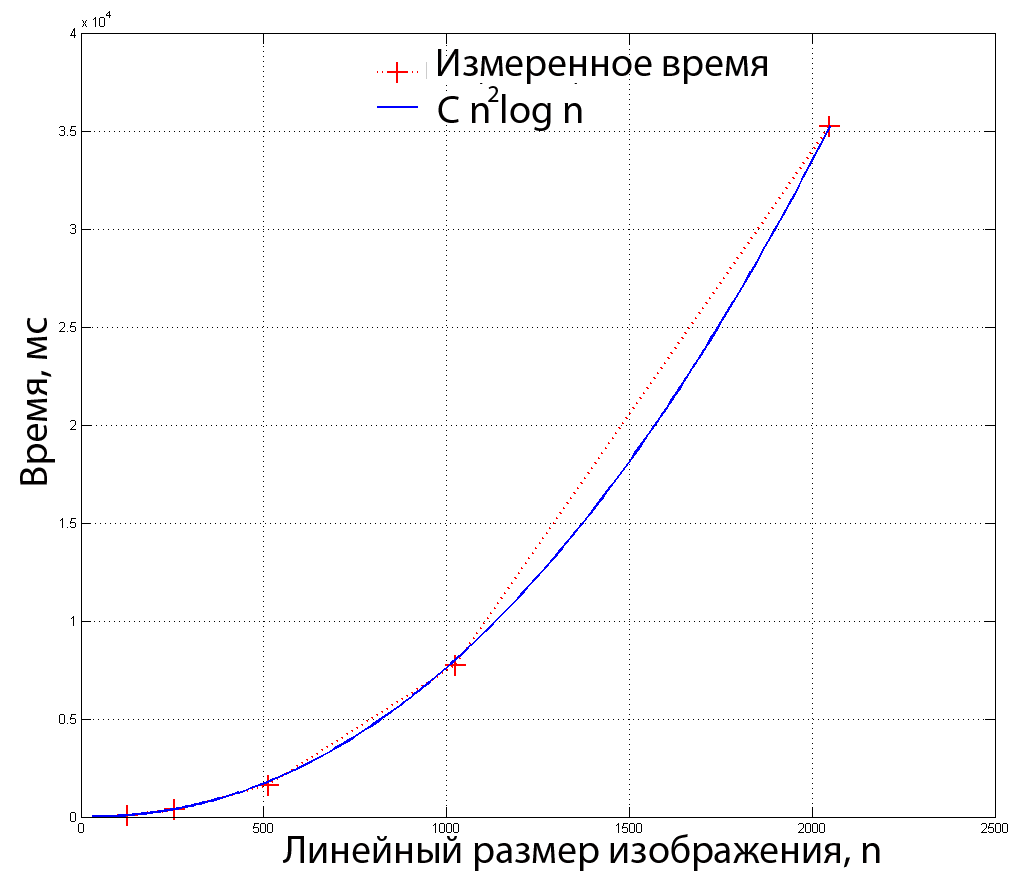
\includegraphics[width=\textwidth]{fht_sirt_time_30_it}
      \caption{Время работы 30 итераций алгоритма}
    \end{figure}
  \end{column}
  \begin{column}{0.6\textwidth}
    \begin{figure}
      \centering
      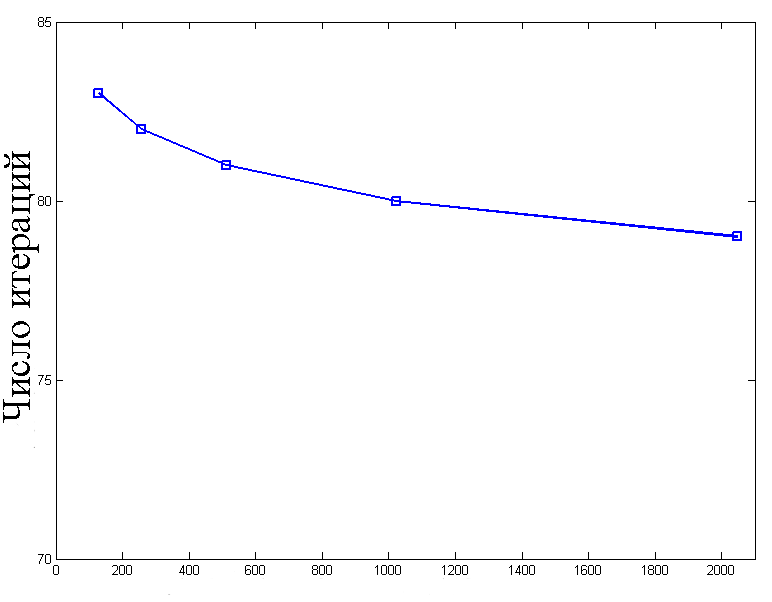
\includegraphics[width=\textwidth]{../Dissertation/images/part1_img/it_till_stop}
      \caption{количество итераций до заданного уровня ошибки на разных размерах изображения}
    \end{figure}
  \end{column}
\end{columns}
\end{frame}

\begin{comment}
\begin{frame}
\frametitle{FHT-SIRT}
\framesubtitle{Предобработка данных}

Перед тем как вести минимизацию с помощью БПХ, необходимо привести измерения в пространство результатов БПХ.
\begin{enumerate}
  \item восстановить соответствие углов проекции строчкам БПХ
  \item растянуть измерения с использованем линейной интерполяции:
\end{enumerate}

\hspace*{2cm}
  \begin{itemize}
    \item \rom{1} растяжение в $\frac 1 {\cos \alpha_i}$ раз
    \item \rom{2} растяжение в $\frac 1 {\cos \alpha_i}$ раз
    \item \rom{3} растяжение в $\frac 1 {\sin \alpha_i}$ раз
    \item \rom{4} растяжение в $\frac 1 {\sin \alpha_i}$ раз
  \end{itemize}

\end{frame}
\end{comment}

\begin{comment}

\begin{frame}
\frametitle{FHT-SIRT}
\framesubtitle{Сходимость при малом количестве углов}
\textbf{Степень разрежения} --- доля отсутствующих углов полного БПХ-пространства
\begin{columns}[T,onlytextwidth]
  \hspace*{-1cm}
  \begin{column}{0.6\textwidth}
  \begin{figure}
    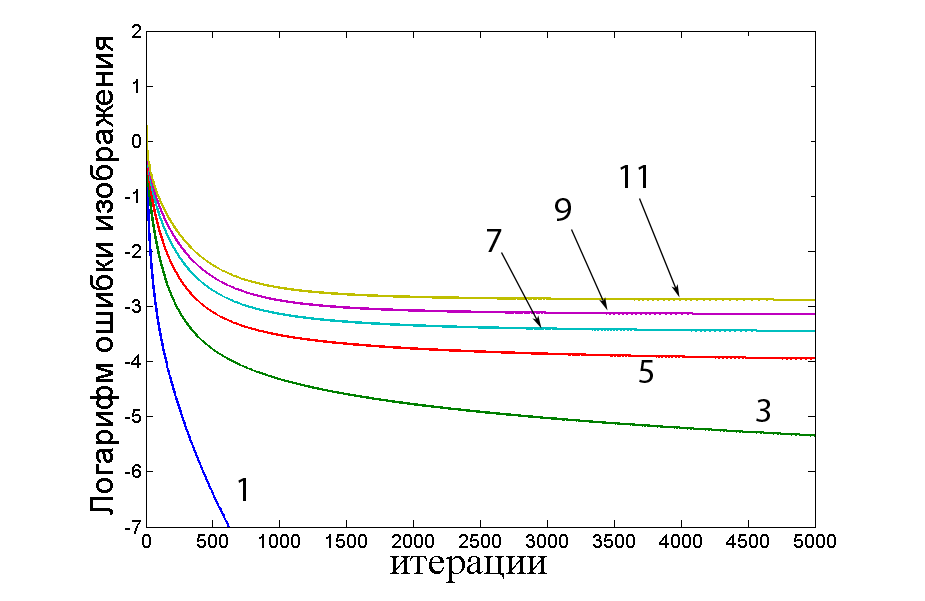
\includegraphics[width=\textwidth]{../Dissertation/images/part1_img/raw}
    \caption{Без регуляризации}
  \end{figure}
  
  \end{column}
  \begin{column}{0.55\textwidth}
    \begin{figure}
    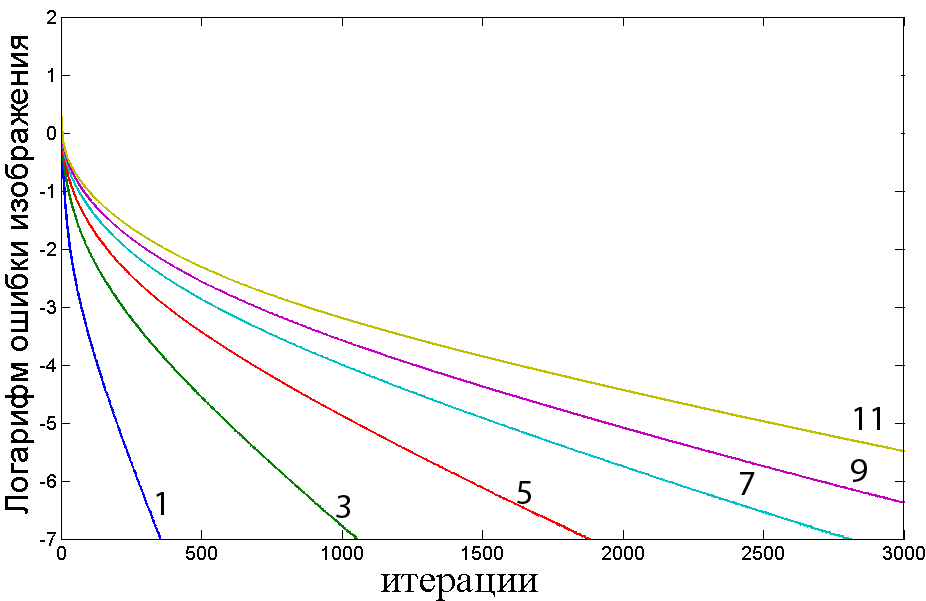
\includegraphics[width=\textwidth]{../Dissertation/images/part1_img/medk}
    \caption{Медианная регуляризация}
    \end{figure}
  \end{column}
\end{columns}
\end{frame}

\begin{frame}
\frametitle{FHT-SIRT}
\framesubtitle{Сходимость при малом количестве углов: медианная регуляризация}

\begin{figure}
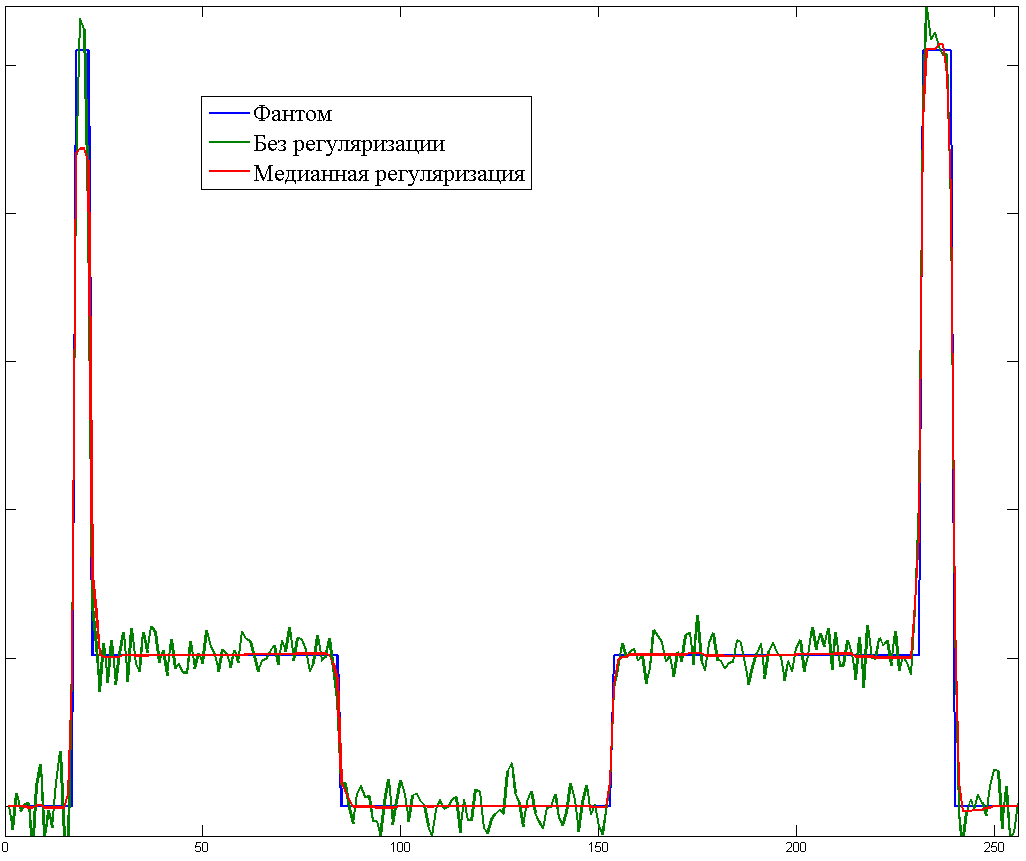
\includegraphics[width=0.8\textwidth]{slice_11}
\end{figure}

\end{frame}
\end{comment}

\begin{comment}
\begin{frame}
\frametitle{FHT-SIRT}
\framesubtitle{Сходимость при малом количестве углов: регуляризация по Тихонову}

    \begin{figure}
    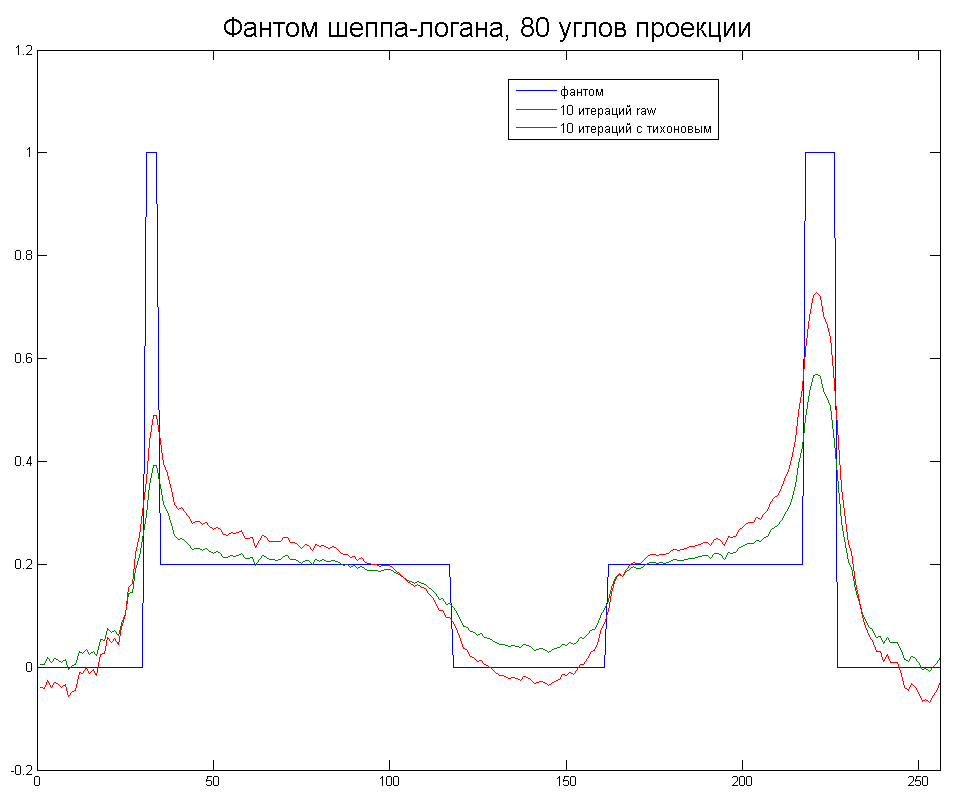
\includegraphics[width=0.8\textwidth]{tikhonov}
    \end{figure}

\end{frame}
\end{comment}

% ======================================================
% ================= Сравнение с SART ===================
% ======================================================
\begin{frame}
\frametitle{FHT-SIRT}
\framesubtitle{сравнение с SART}
  \begin{figure}
  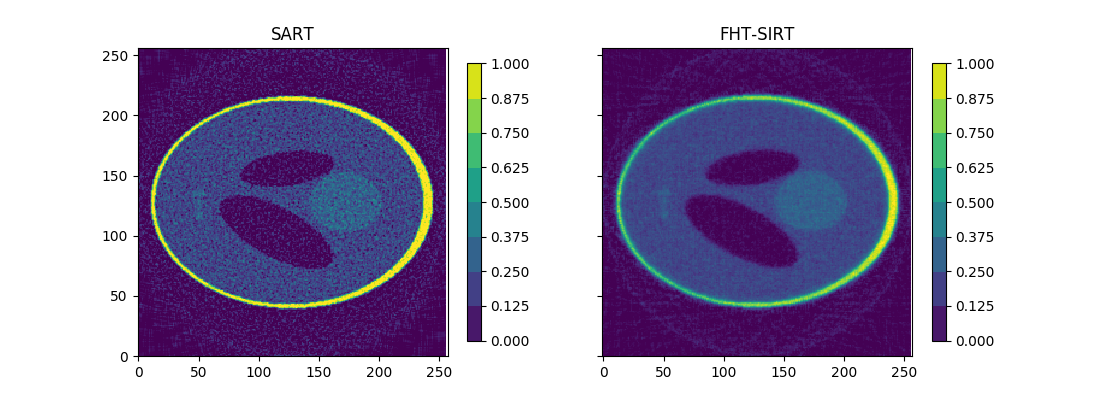
\includegraphics[width=0.8\textwidth]{sart__fht_sirt}
  \end{figure}

% \hline
\vspace{0.5cm}


\small
\begin{tabular}{c|c c}
    метод & SART & FHT-SIRT \\ \vspace{5pt}
    количество итераций & 1 & 40 \\ \vspace{5pt}
    время & 0.931c & 0.935c \\ \vspace{5pt}
    ошибка & 11.8845 & 16.1192 \\ \vspace{5pt}
    СКО & 0.3278 & 0.3882 \\ \vspace{5pt}
    N & 256 & 256 \\
\end{tabular}

\end{frame}


\begin{frame}
\frametitle{FHT-SIRT}
\framesubtitle{сравнение с SART: кросс-секции}
\begin{columns}[T,onlytextwidth]
  \hspace*{-1cm}
  \begin{column}{0.2\textwidth}
    \begin{figure}
      \centering
      \vspace{1.5cm}
      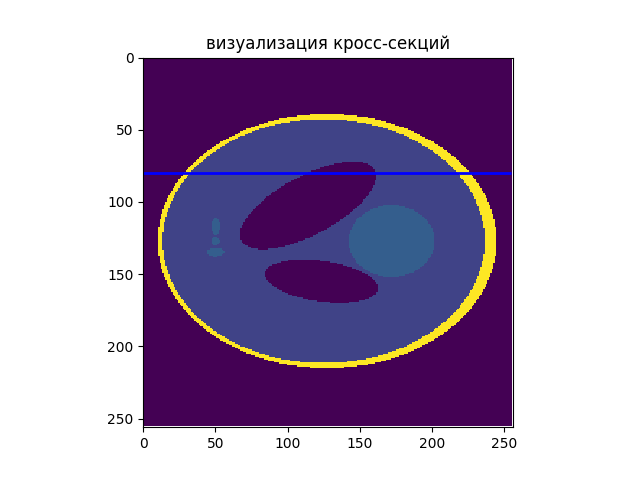
\includegraphics[width=1.5\textwidth]{cs_80_viz}
    \end{figure}
  \end{column}
  \begin{column}{0.8\textwidth}
    \begin{figure}
      \centering
      \vspace{-1cm}
      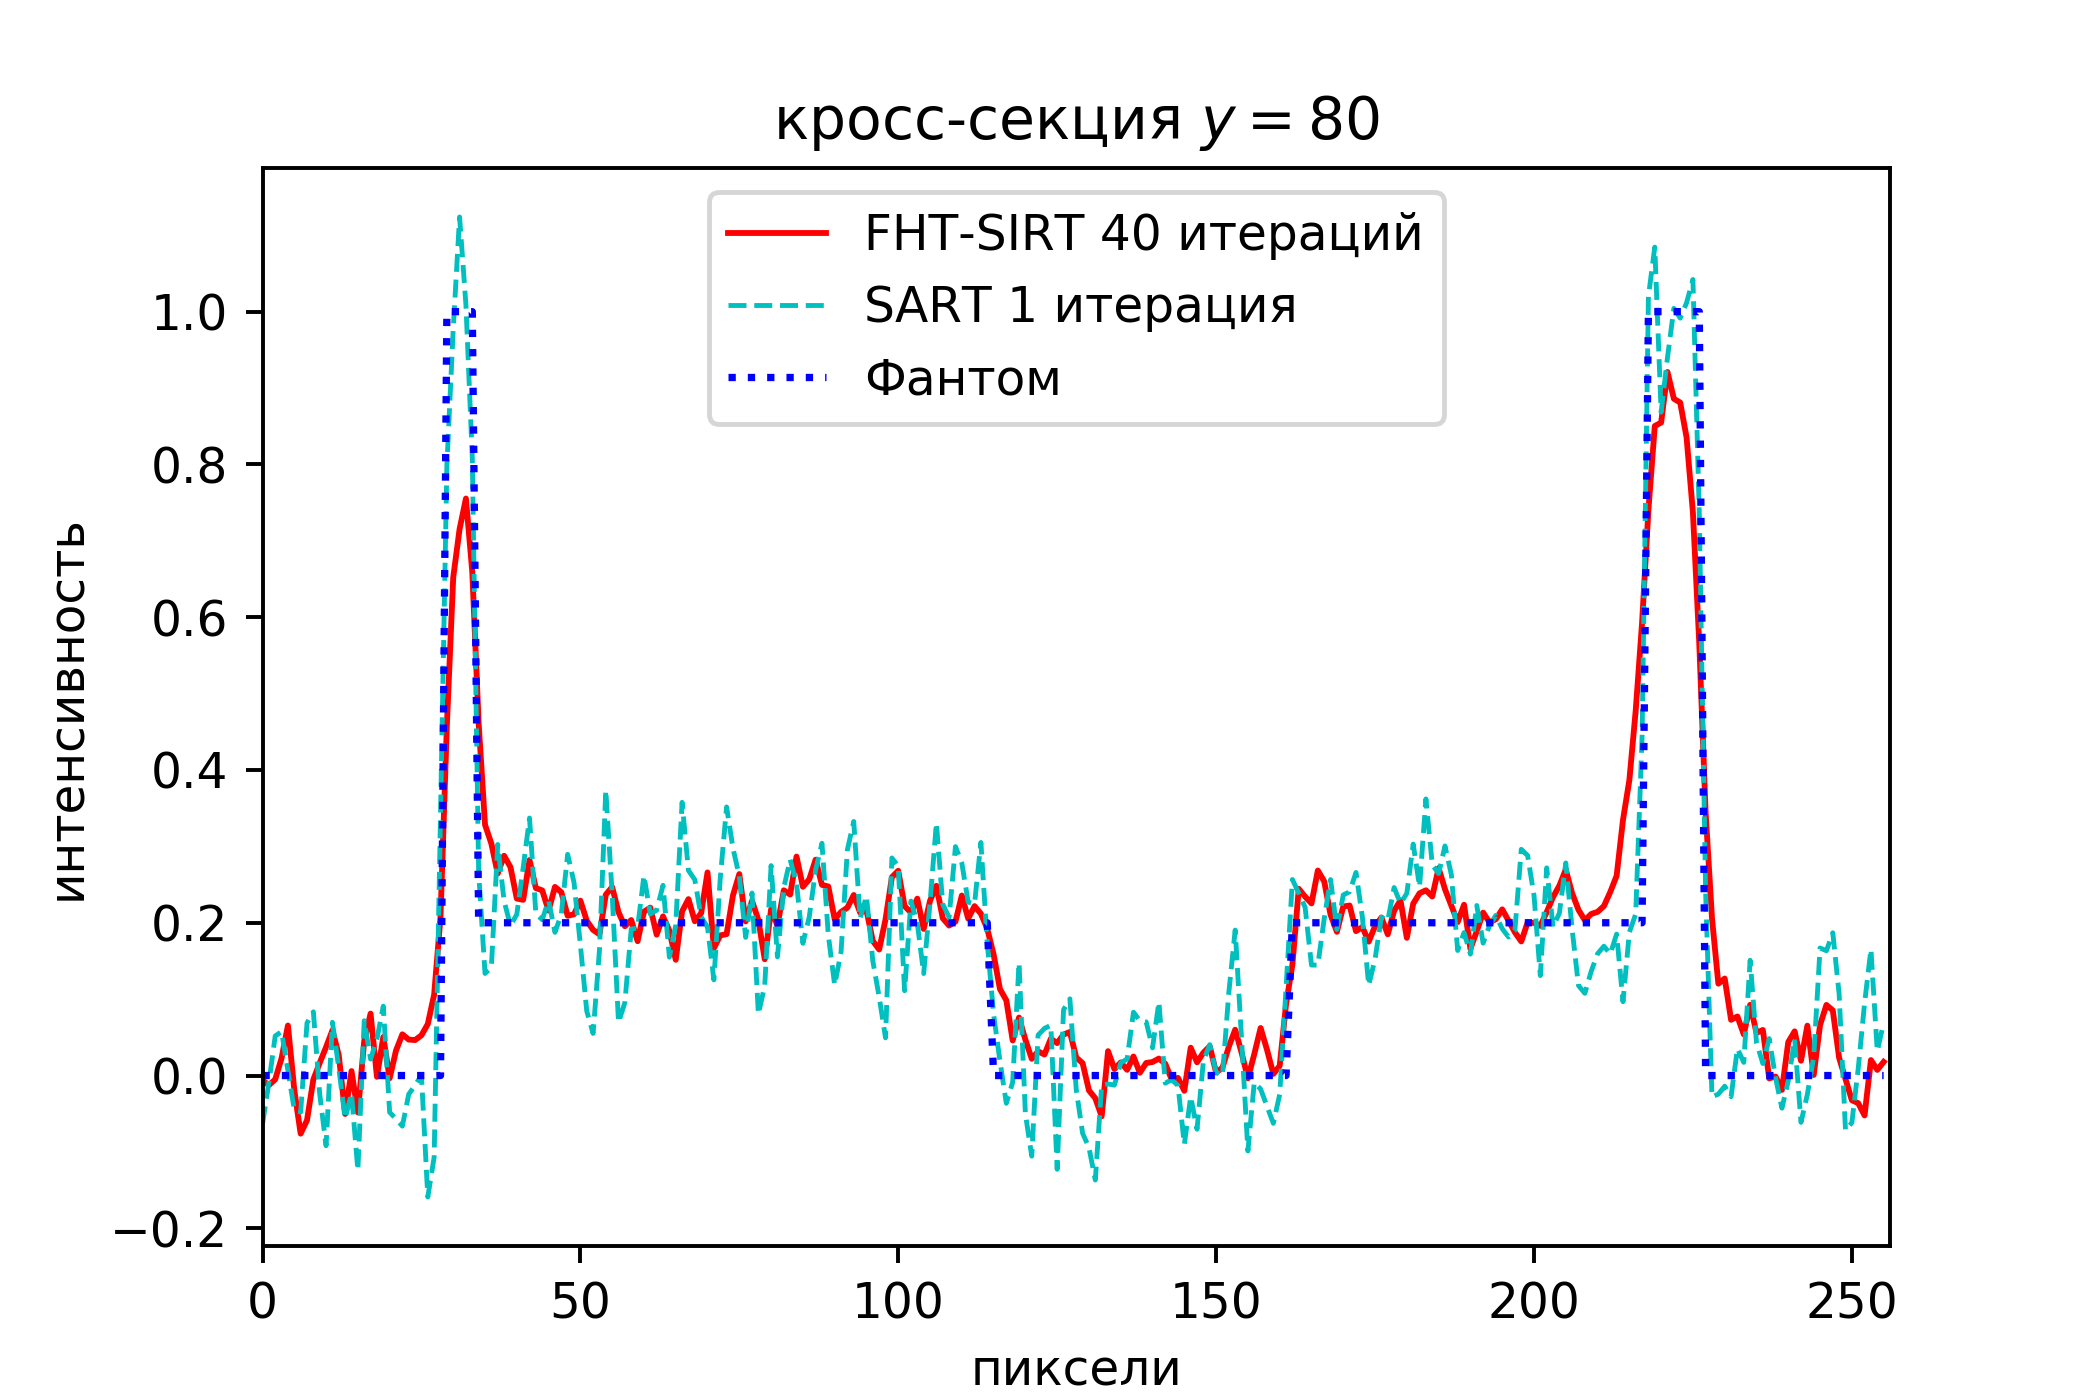
\includegraphics[width=1.2\textwidth]{cs_80}
    \end{figure}
  \end{column}
\end{columns}
\end{frame}

\begin{frame}
\frametitle{FHT-SIRT}
\framesubtitle{сравнение с SART: кросс-секции}
\begin{columns}[T,onlytextwidth]
  \hspace*{-1cm}
  \begin{column}{0.2\textwidth}
    \begin{figure}
      \centering
      \vspace{1.5cm}
      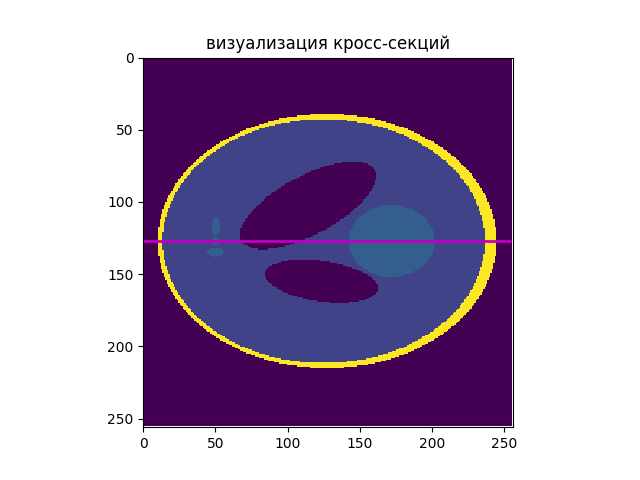
\includegraphics[width=1.5\textwidth]{cs_127_viz}
    \end{figure}
  \end{column}
  \begin{column}{0.8\textwidth}
    \begin{figure}
      \centering
      \vspace{-1cm}
      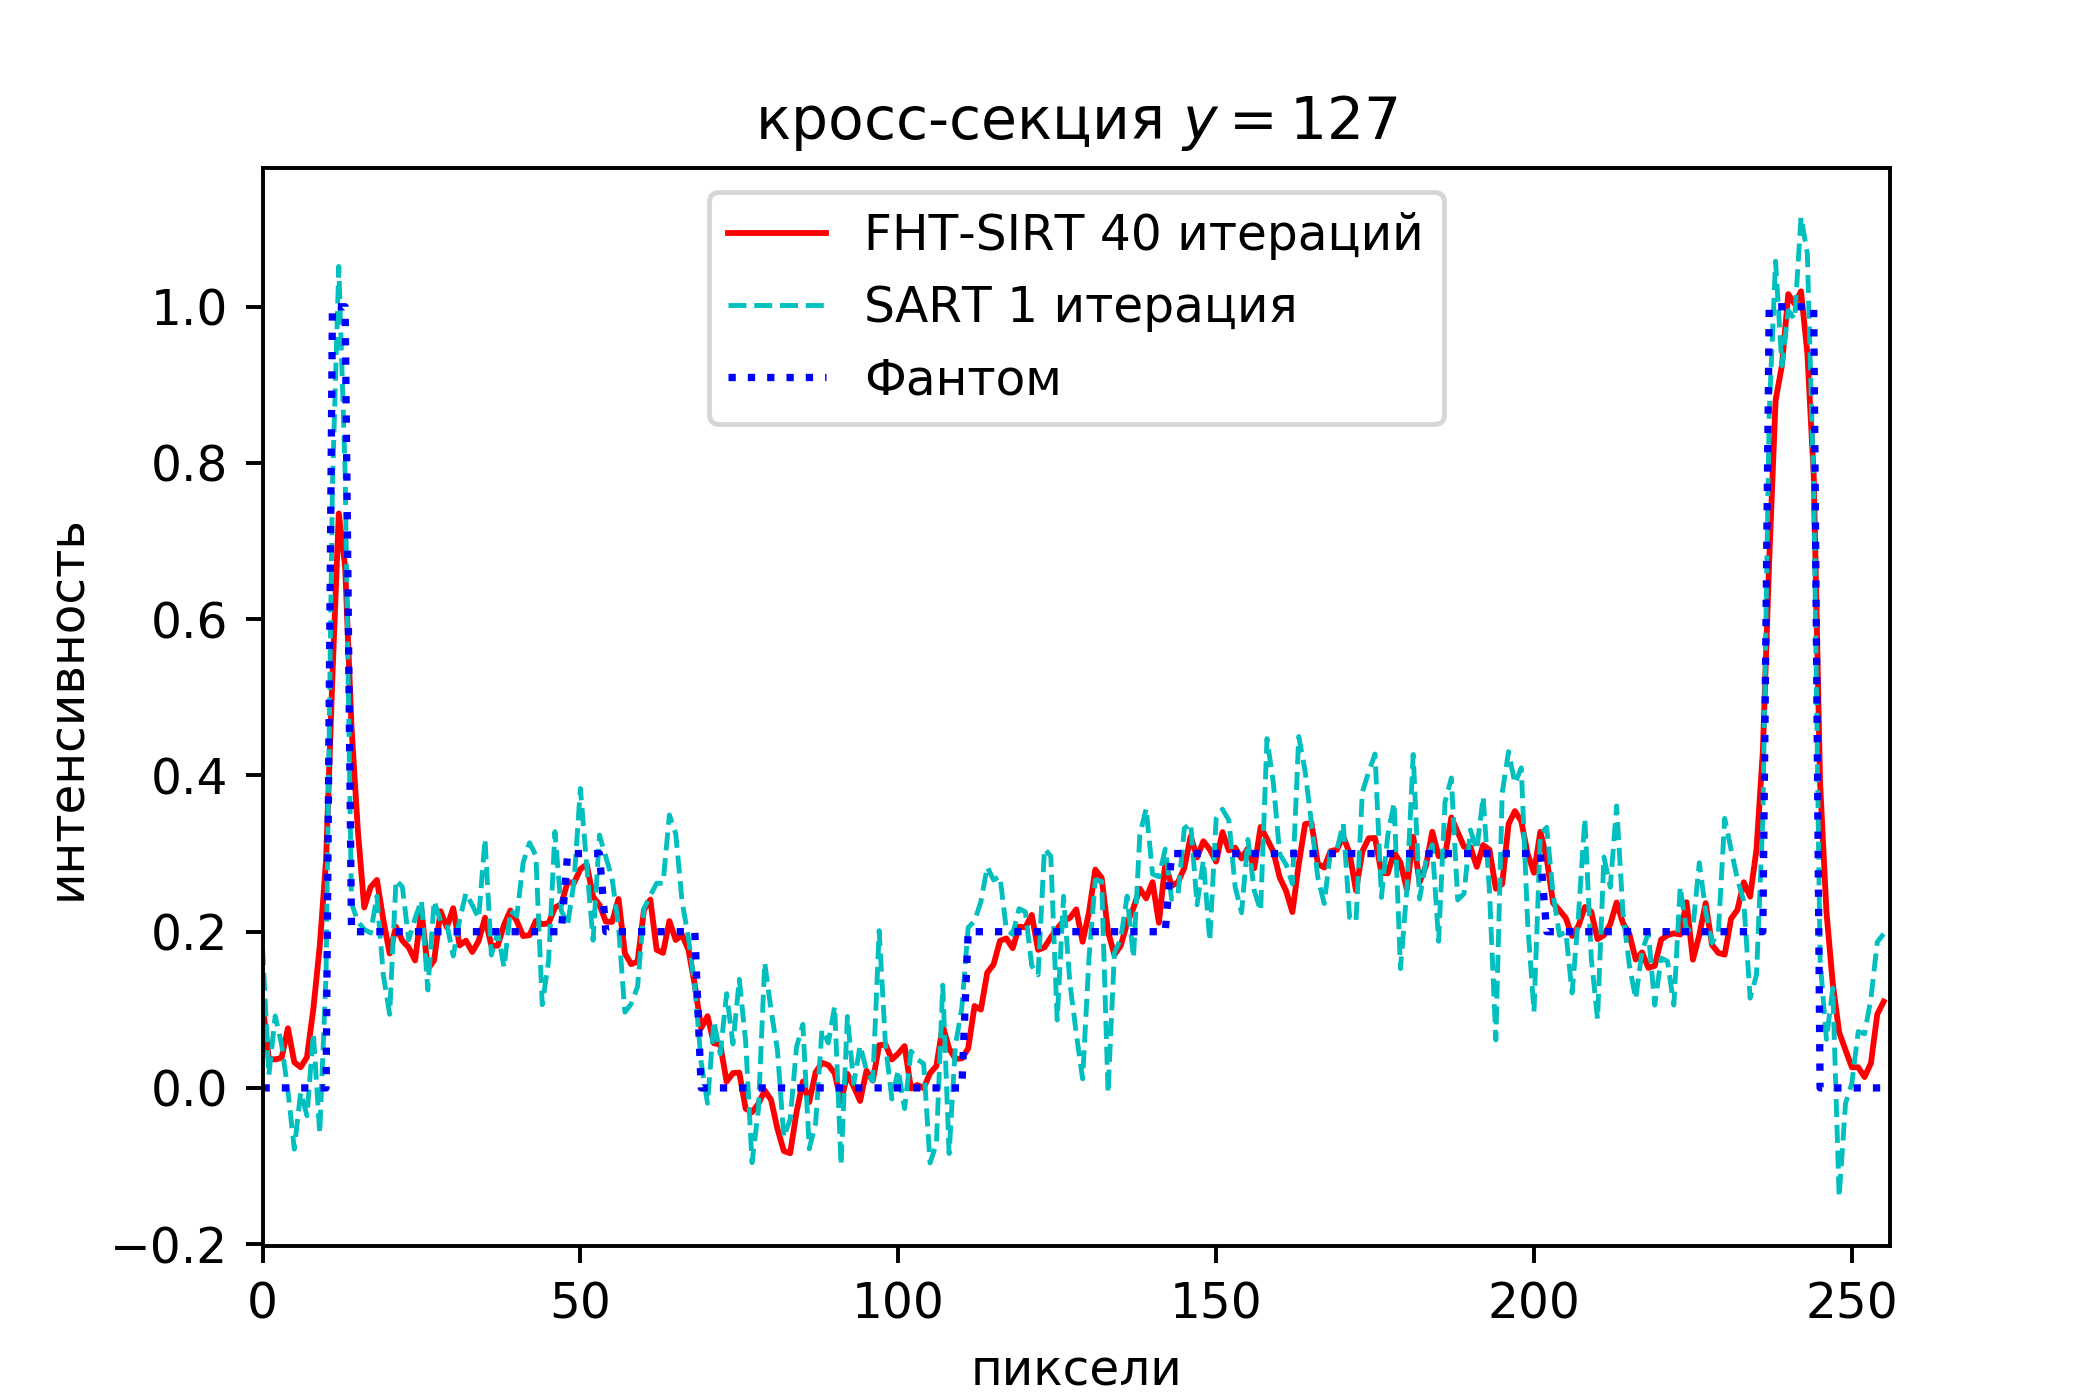
\includegraphics[width=1.2\textwidth]{cs_127}
    \end{figure}
  \end{column}
\end{columns}
\end{frame}


\begin{frame}
\frametitle{FHT-SIRT}
\framesubtitle{сравнение с SART: кросс-секции}
\begin{columns}[T,onlytextwidth]
  \hspace*{-1cm}
  \begin{column}{0.2\textwidth}
    \begin{figure}
      \centering
      \vspace{1.5cm}
      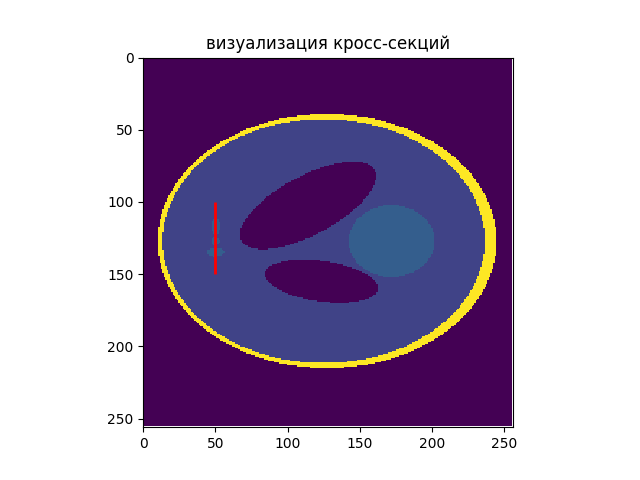
\includegraphics[width=1.5\textwidth]{cs_v_50_viz}
    \end{figure}
  \end{column}
  \begin{column}{0.8\textwidth}
    \begin{figure}
      \centering
      \vspace{-1cm}
      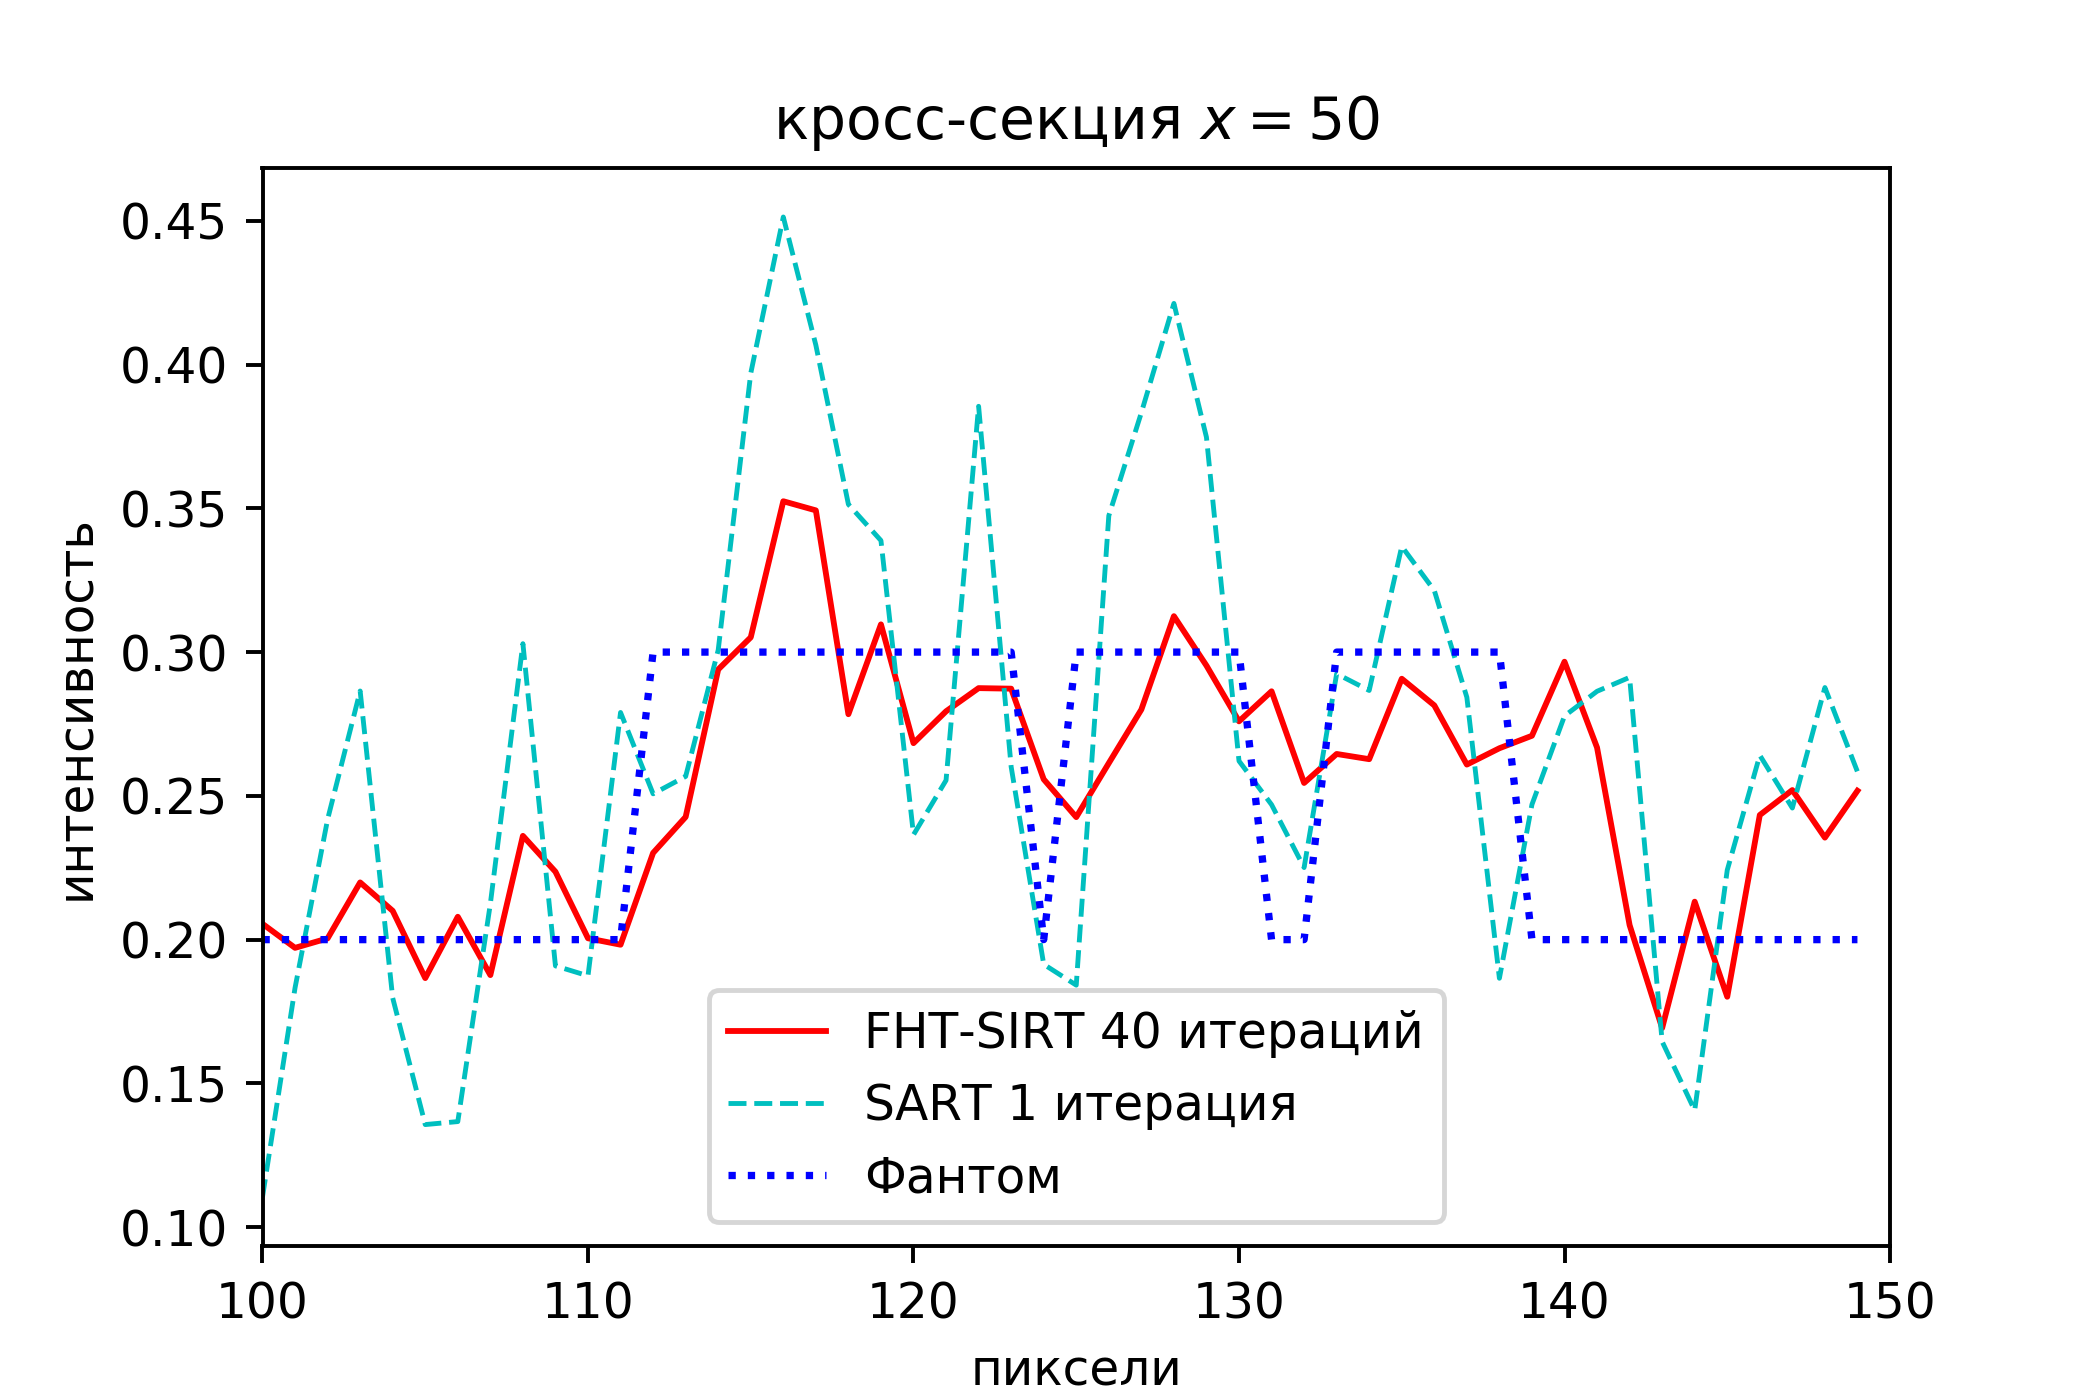
\includegraphics[width=1.2\textwidth]{cs_v_50}
    \end{figure}
  \end{column}
\end{columns}
\end{frame}


\begin{frame}
\frametitle{Выводы}
\begin{itemize}
  \item Построен асимптотически эффективный алгоритм вычисления обратной проекций с помощью быстрого преобразования Хафа (БПХ)
  \item Использование БПХ позволяет снизить асимпотику итерации метода SIRT с $O(N^3)$ до $O(N^2 \log N)$
  \item Построенный алгоритм FHT-SIRT позволяет добиться качества восстановления, аналогичного качеству традиционных алгоритмов
\end{itemize}
\end{frame}

\section{Подавление артефактов, вызванных наличием сильнопоглощающих включений}
% \section{Подавление артефактов, вызванных наличием сильнопоглощающих включений}

\begin{frame}
\frametitle{Примеры артефактов}

\begin{columns}[t]
\column{.5\textwidth}
\centering
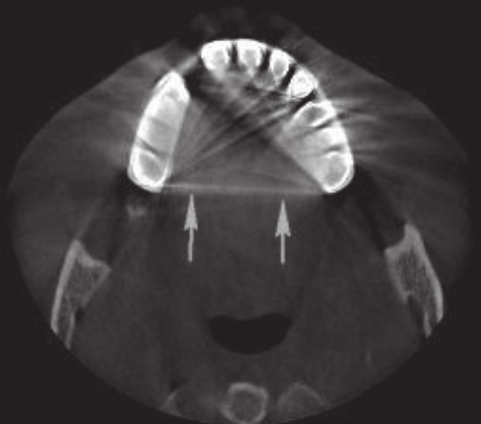
\includegraphics[height=0.5\textheight]{../Dissertation/images/part2_img/tooth_artifacts_med}\\
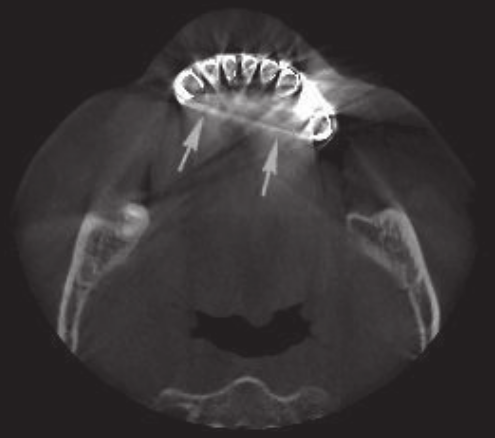
\includegraphics[height=0.5\textheight]{../Dissertation/images/part2_img/tooth_artifacts_med_2}

\column{.5\textwidth}
\centering
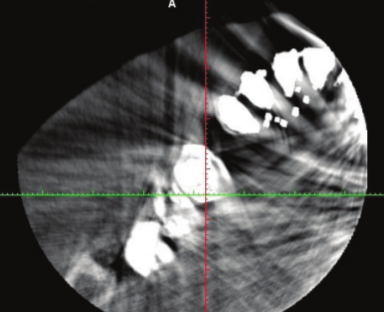
\includegraphics[height=0.5\textheight]{../Dissertation/images/part2_img/tooth_artifacts_med_3}\\
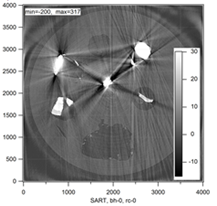
\includegraphics[height=0.5\textheight]{high_absorb_artifacts}
\end{columns}

\end{frame}

\begin{frame}
\frametitle{Модель возникновения артефактов}
  \begin{itemize}[<+->]
    \item при прохождении через сильнопоглощающие включения большая часть излучения поглощается
    \item пиксели детектора имеют некоторый порог активации $\delta_{\mathrm I min}$
    \item если пришедшая интетсивность $\mathrm I_{j} \leq \delta_{\mathrm I min}$, показание детектора будет неотличимо от уровня шума
    \item оптимизационная задача должна учитывать такие измерения особым образом
    \item при логарифмировании условие $\mathrm I_{j} \leq \delta_{\mathrm I min}$ переходит в 
    \begin{equation}
      \label{eq:thresh}
      p_j \geq \delta \left( = \ln \frac {\mathrm I_0}{\delta_{\mathrm I min}}\right)
    \end{equation}
  \end{itemize}
\end{frame}



\begin{frame}
\frametitle{Учет пикселей с высоким поглощением}
Пусть $\mathbb J = \left\{ j | p_j \geq \delta \right\}$, то есть индексы пикселей, для которых выполнено условие (\ref{eq:thresh}).

С учетом пороговой активации, а так же неотрицательности функции $f$, оптимизационная задача будет иметь вид:


\begin{equation} \notag
  % \label{eq:quadprog_ineq}
  \begin{cases}
  \Norm{p - Wf} \rightarrow \min\limits_f & w.r.t \\
  \sum_i f_{i} \omega_{ij} > \delta, & \mbox{если } j \in \mathbb J \\
  f_{i} \geq 0 & \\
  \end{cases}
\end{equation}

\end{frame}


\begin{frame}
\frametitle{Квадратичное программирование}
\begin{itemize}
  \item оптимизация квадратичной функции на наборе линейных ограничений
  \item частный случай выпуклой оптимизации
  \item требует обращения матрицы $W^{\mathrm T} W$. 
  \item для изображения 256х256 и 180 углов при использовании float64 такая матрица будет занимать порядка 32Гб
\end{itemize}


\end{frame}

\begin{frame}
\frametitle{Применение qp для малых размерностей}
\begin{columns}[T,onlytextwidth]
  \hspace*{-1cm}
\begin{column}{0.4\textwidth}
  \begin{figure}
    \centering
    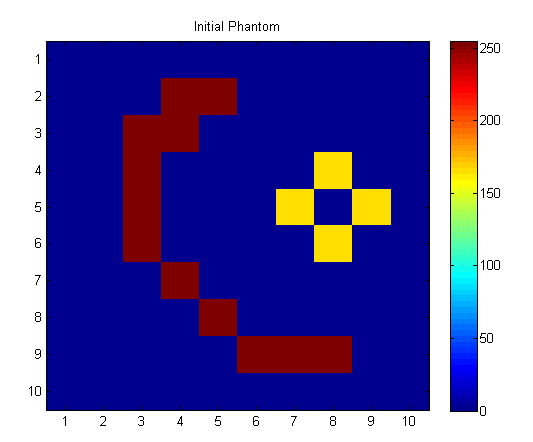
\includegraphics[width=\textwidth]{qp_phantom}
  \end{figure}
  фантом
\end{column}

\begin{column}{0.4\textwidth}
  \begin{figure}
    \centering
    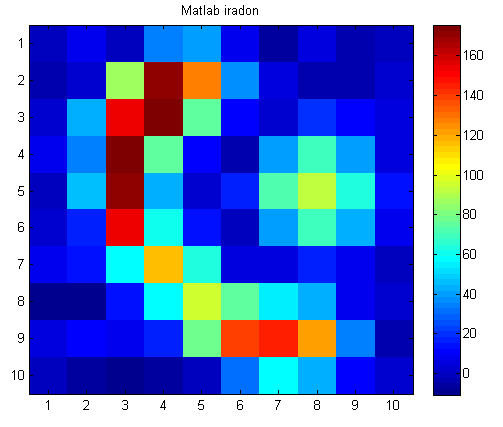
\includegraphics[width=\textwidth]{qp_fbp}
  \end{figure}
  matlab iradon (fpb)
\end{column}

\begin{column}{0.4\textwidth}
    \begin{figure}
    \centering
    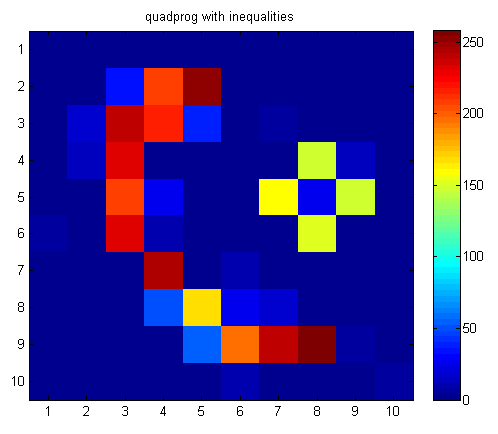
\includegraphics[width=\textwidth]{qp_qp_ineq}
  \end{figure}
  QP с ограничениями-неравенствами
\end{column}
\end{columns}

\end{frame}

\begingroup
\small
\begin{frame}
  \frametitle{Как повысить разрешение?}
  \begin{columns}[T, onlytextwidth]
  \hspace{-0.5cm}
  \begin{column}{0.5\textwidth}
    \underline{Метод мягких неравенств} \\ \vspace{0.5cm}
    Введем диагональную матрицу $\mathrm J \in \textup{diag}\{N N_\varphi\}$, такую что 
    $\mathrm J_{j} = \left\{1, \mbox{если}\ j \in \mathbb J, \mbox{иначе }\ 0\right\}$, а так же $\mathrm K = \mathrm E - \mathrm J$.


    \begin{equation} \notag
      \label{eq:soft-ineq}
      \begin{array}{lc}
      \Norm{K(Wf - p)}^2 & + \\
      \alpha \Norm{J(Wf - \delta)_{+}}^2  & \to \min\limits_f
      \end{array}
    \end{equation}
  \end{column}

  \begin{column}{0.5\textwidth}
    \underline{Метод барьерных функций} \\ \vspace{0.5cm}
    Заменим неравенства вида $g(x) \leq 0$ на аддитивные барьерные функции $-\frac 1 t \log{\left(-g(x)\right)}$.
    Начиная из ``внутренней''точки, будем минимизировать функционал, постепенно увеличивая t.
    $$
    \begin{array}{ccc}
      F_t(f) = & \Norm{Wf - p}^2 & + \\
     \frac 1 t \sum \left( -\log{\left(-g(x)\right)} \right) &\to \min\limits_f &
    \end{array}{ccc}
    $$

    Так же возможно ввести ослабить ограничения, добавив переменные нежесткости $\xi$

  \end{column}
  \end{columns}
\end{frame}
\endgroup

\begin{frame}
\frametitle{Метод мягких неравенств}
\framesubtitle{фантом}

\begin{figure}
  \centering
  \vspace{-0.3cm}
  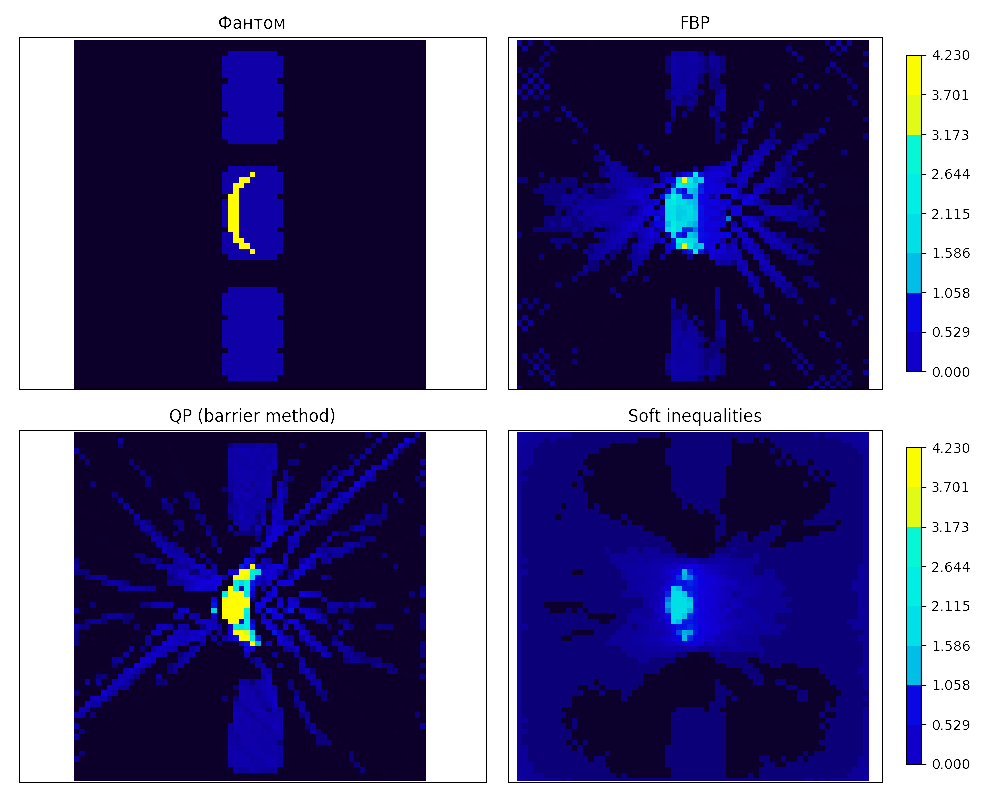
\includegraphics[height=0.7\textheight]{qp_foursome}
  \caption{сравнение реконструкции различными методами}
  \label{fig:sample}
\end{figure}

\end{frame}


\begin{frame}
\frametitle{Метод мягких неравенств}
\framesubtitle{другая палитра}

\begin{figure}
  \centering
  \vspace{-0.3cm}
  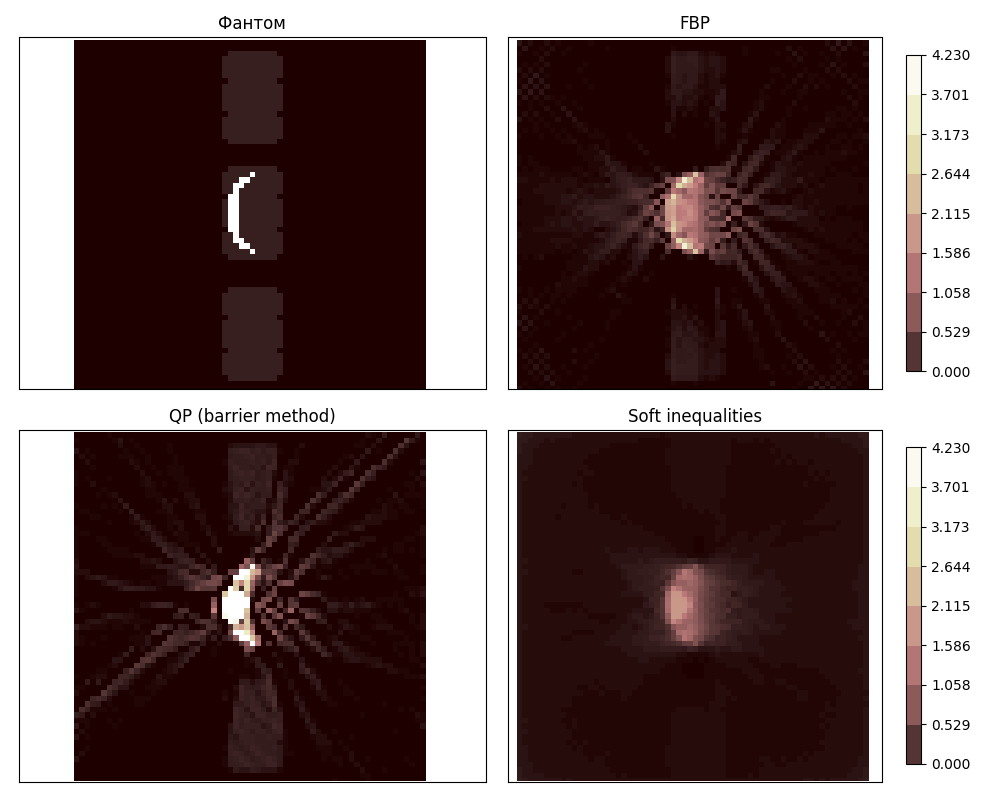
\includegraphics[height=0.7\textheight]{qp_foursome_pink}
  \caption{сравнение реконструкции различными методами}
  \label{fig:sample}
\end{figure}

\end{frame}

\begin{frame}
\frametitle{Метод мягких неравенств}
\framesubtitle{реконструкция экспериментальных данных}

\begin{figure}
\centering
\vspace{-0.3cm}
\begin{tabular}{@{}c@{}c}
    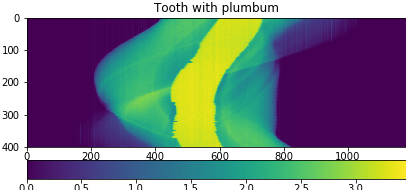
\includegraphics[width=0.50\textwidth]{../Dissertation/images/part2_img/tooth_sino}
&
    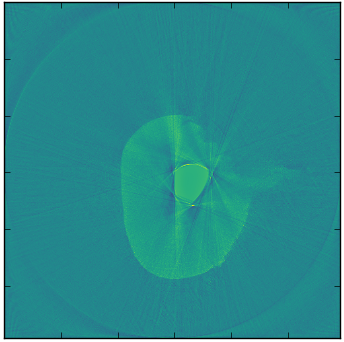
\includegraphics[width=0.50\textwidth]{../Dissertation/images/part2_img/soft_ineq_pb_tooth}
\\
   \small a) & \small b)
\end{tabular}
  \caption{a --- Синограмма молочного зуба с включением из свинца. б --- результат восстановления методом мягких ограничений}
\label{fig:tooth_sino_rec}
\end{figure}

\end{frame}

\section{Задача реконструкции при зондировании полихроматическим излучением}
%\section{Задача реконструкции при зондировании полихроматическим излучением}

\begingroup
\small
\begin{frame}
\frametitle{Модель измерений}

При переходе к немонохроматическому случаю, уравнение затухания прошедшей через объект интенсивности: 
\begin{equation}
\notag
I(\varphi, \xi) = \int_0^{+\infty}{\left\{
  I_0(\lambda) \exp{\left(- {\mathrm R}[f(\lambda)](\varphi, \xi) \right)} d\lambda
  \right\}}  
\end{equation}


Будем считать, что объект состоит из $K$ элементов, с неизвестными пространственными концентрациями $c_k(x,y)$, и известными табулированными массовыми коэффициентами ослабления $\kappa_k(\lambda)$.
Тогда
$$
f(x,y, \lambda) = \sum_{k = 1} ^K {c_k(x,y) * \kappa_k(\lambda)}
$$

и прямая проекция для пикселя $j$ принимает вид

\begin{equation} \notag
  \label{eq:white_fp_final}
  I(c)_j = \int_0^{+\infty} {d\lambda \left\{
    I_0(\lambda) \exp{\left(
      -\sum_{k=1}^K {\rho \kappa_k(\lambda) (W c_k)_j} 
      \right)}
  \right\}}
\end{equation}

\end{frame}
\endgroup

\begin{frame}
\frametitle{Оптимизационная задача}

Следуя алгебраическому подходу, реконструкция проводится с помощью градиентного спуска оптимизации квадратичной функции потерь 
$$
Q(c) = \frac {\left(I(c) - t\right)^2} {S} \to \min \limits_c,
$$
где $t$ --- измеренные интенсивности прошедшего через объект излучения, \\
$S = \left( \int_0^{+\infty} { I_0(\lambda) d\lambda} \right)^2$
 --- суммарная интенсивность зондирующего излучения.

\end{frame}

\begin{frame}
\frametitle{Градиент функции потерь}
\begin{equation} \notag
\label{eq:part3_whitegrad}
  \nabla_k \ Q = 2W^\intercal R_k \text{, где } R_{kj} = \frac {(I(c) - t)_j} {S} \mu_{kj}
\end{equation}

а формулы для вычисления весов невязок по каждому элементу приведены ниже:
\begin{equation} \notag
  \label{eq:weights}
  \mu_{k} = \int_0^{+\infty} {d\lambda \left\{
    -\rho \kappa_k(\lambda) 
    I_0(\lambda)
    \exp{\left(
      -\sum_{s=1}^K {\rho \kappa_s(\lambda) (W c_s)} 
         \right)}
    \right\}}
\end{equation}

\end{frame}


\begin{frame}
\frametitle{Метод взвешенных невязок}
\framesubtitle{регуляризация}
  \begin{block}{Мультипликативная регуляризация}
    Запрещаем одновременное нахождение разных элементов в одном пикселе, т.е. $c_{k} \odot c_{s} = 0 \mbox{, если} k \neq s$.

    $$
    Q(c) + \beta\sum_{k_1 != k_2}\Norm{c_{k_1} \odot c_{k_2}} \to \min \limits_c
    $$
  \end{block}
  \begin{block}{Ограничение на значения концентраций}
  Используя метод барьерных функций, можем учесть, что концентрации имеют значения на интервале $[0, 1]$
    $$
    \begin{array}{lc}
    Q(c) \to \min \limits_c & w.r.t \\
    c_k \geq 0 & \\
    c_k \leq 1
    \end{array}
    $$
  \end{block}
\end{frame}

\begin{frame}
\frametitle{Исходные данные}
\begin{figure}
\centering
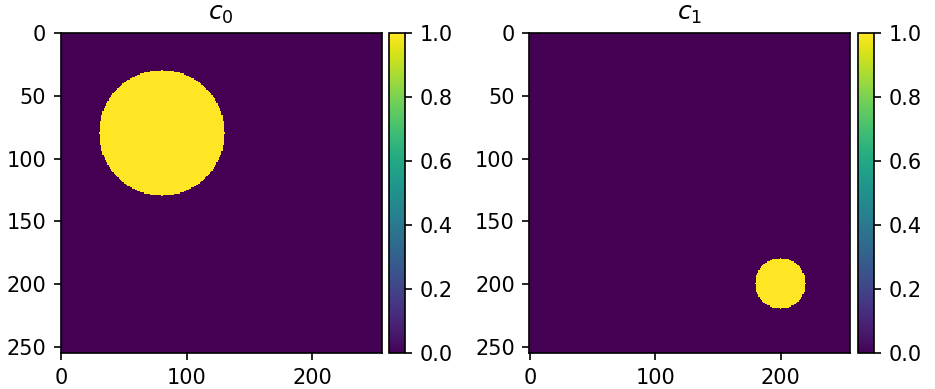
\includegraphics[width=\textwidth]{0999}
\\
\caption{фантом на тривиальных спектрах}
\end{figure}
\end{frame}


\begin{frame}
\frametitle{Исходные данные}
\begin{figure}

\centering
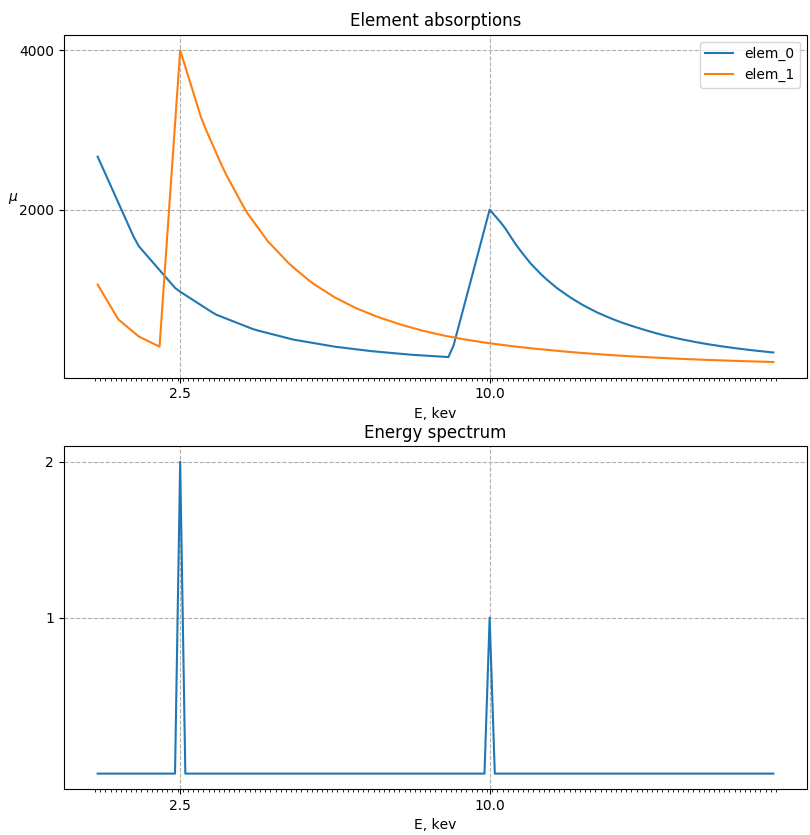
\includegraphics[height=0.7\textheight]{../Dissertation/images/part3_img/synth_spectre}
\\
\caption{спектры и массовые коэффициенты ослабления элементов}
\end{figure}

\end{frame}

\begin{frame}
\frametitle{Результаты восстановления}
\begin{figure}
\centering
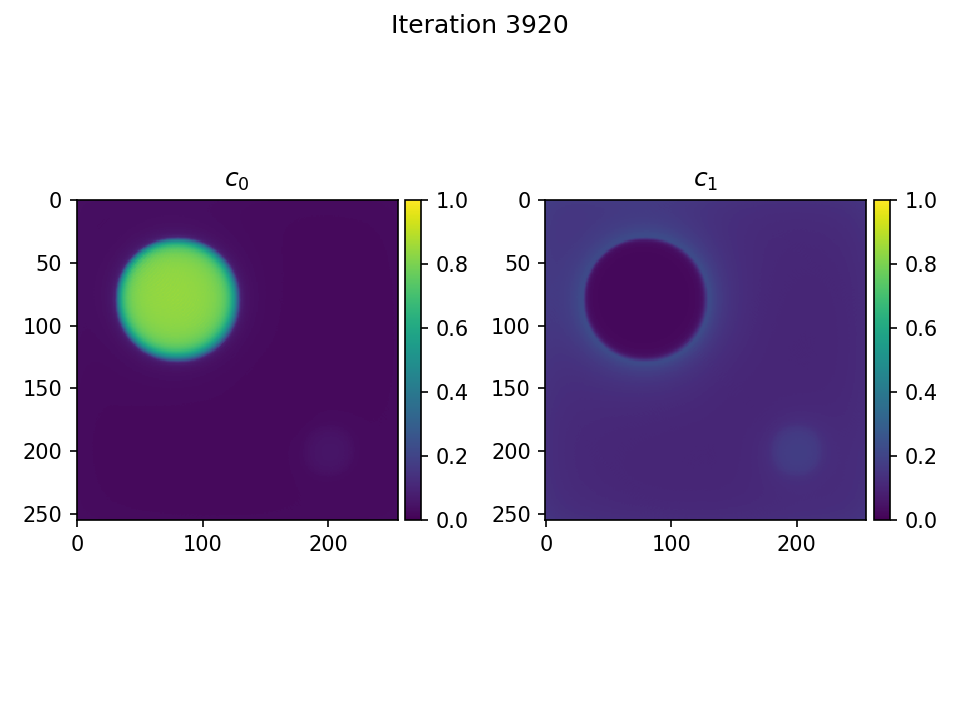
\includegraphics[width=\textwidth]{whiterec_res}
\\
\caption{Метод взвешенных невязок + метод барьерных функций + мультипликативная регуляризация}
\end{figure}
\end{frame}

\begin{frame}
\frametitle{Реальные экспериметнальные данные}
\centering
\vspace{-0.3cm}
\begin{columns}

\begin{column}{0.2\textwidth}
\begin{figure}
    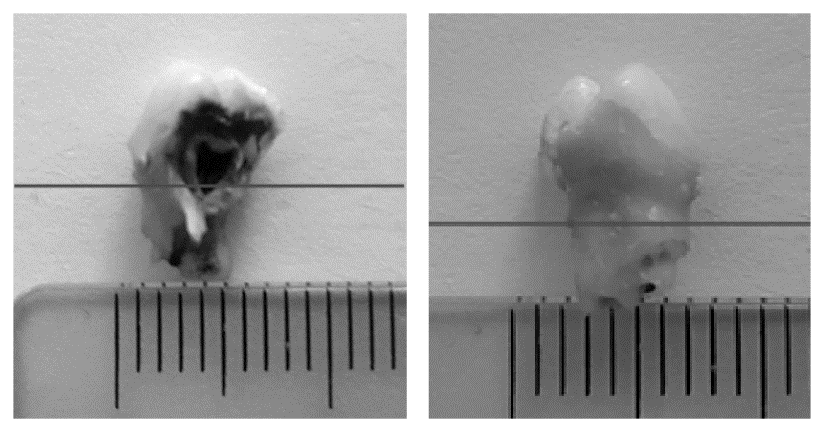
\includegraphics[width=1\textwidth]{zub_photo}
    \caption{зуб (Ca) с включением из свинца (Pb)}
\end{figure}
\end{column}

\begin{column}{0.8\textwidth}
\begin{figure}
    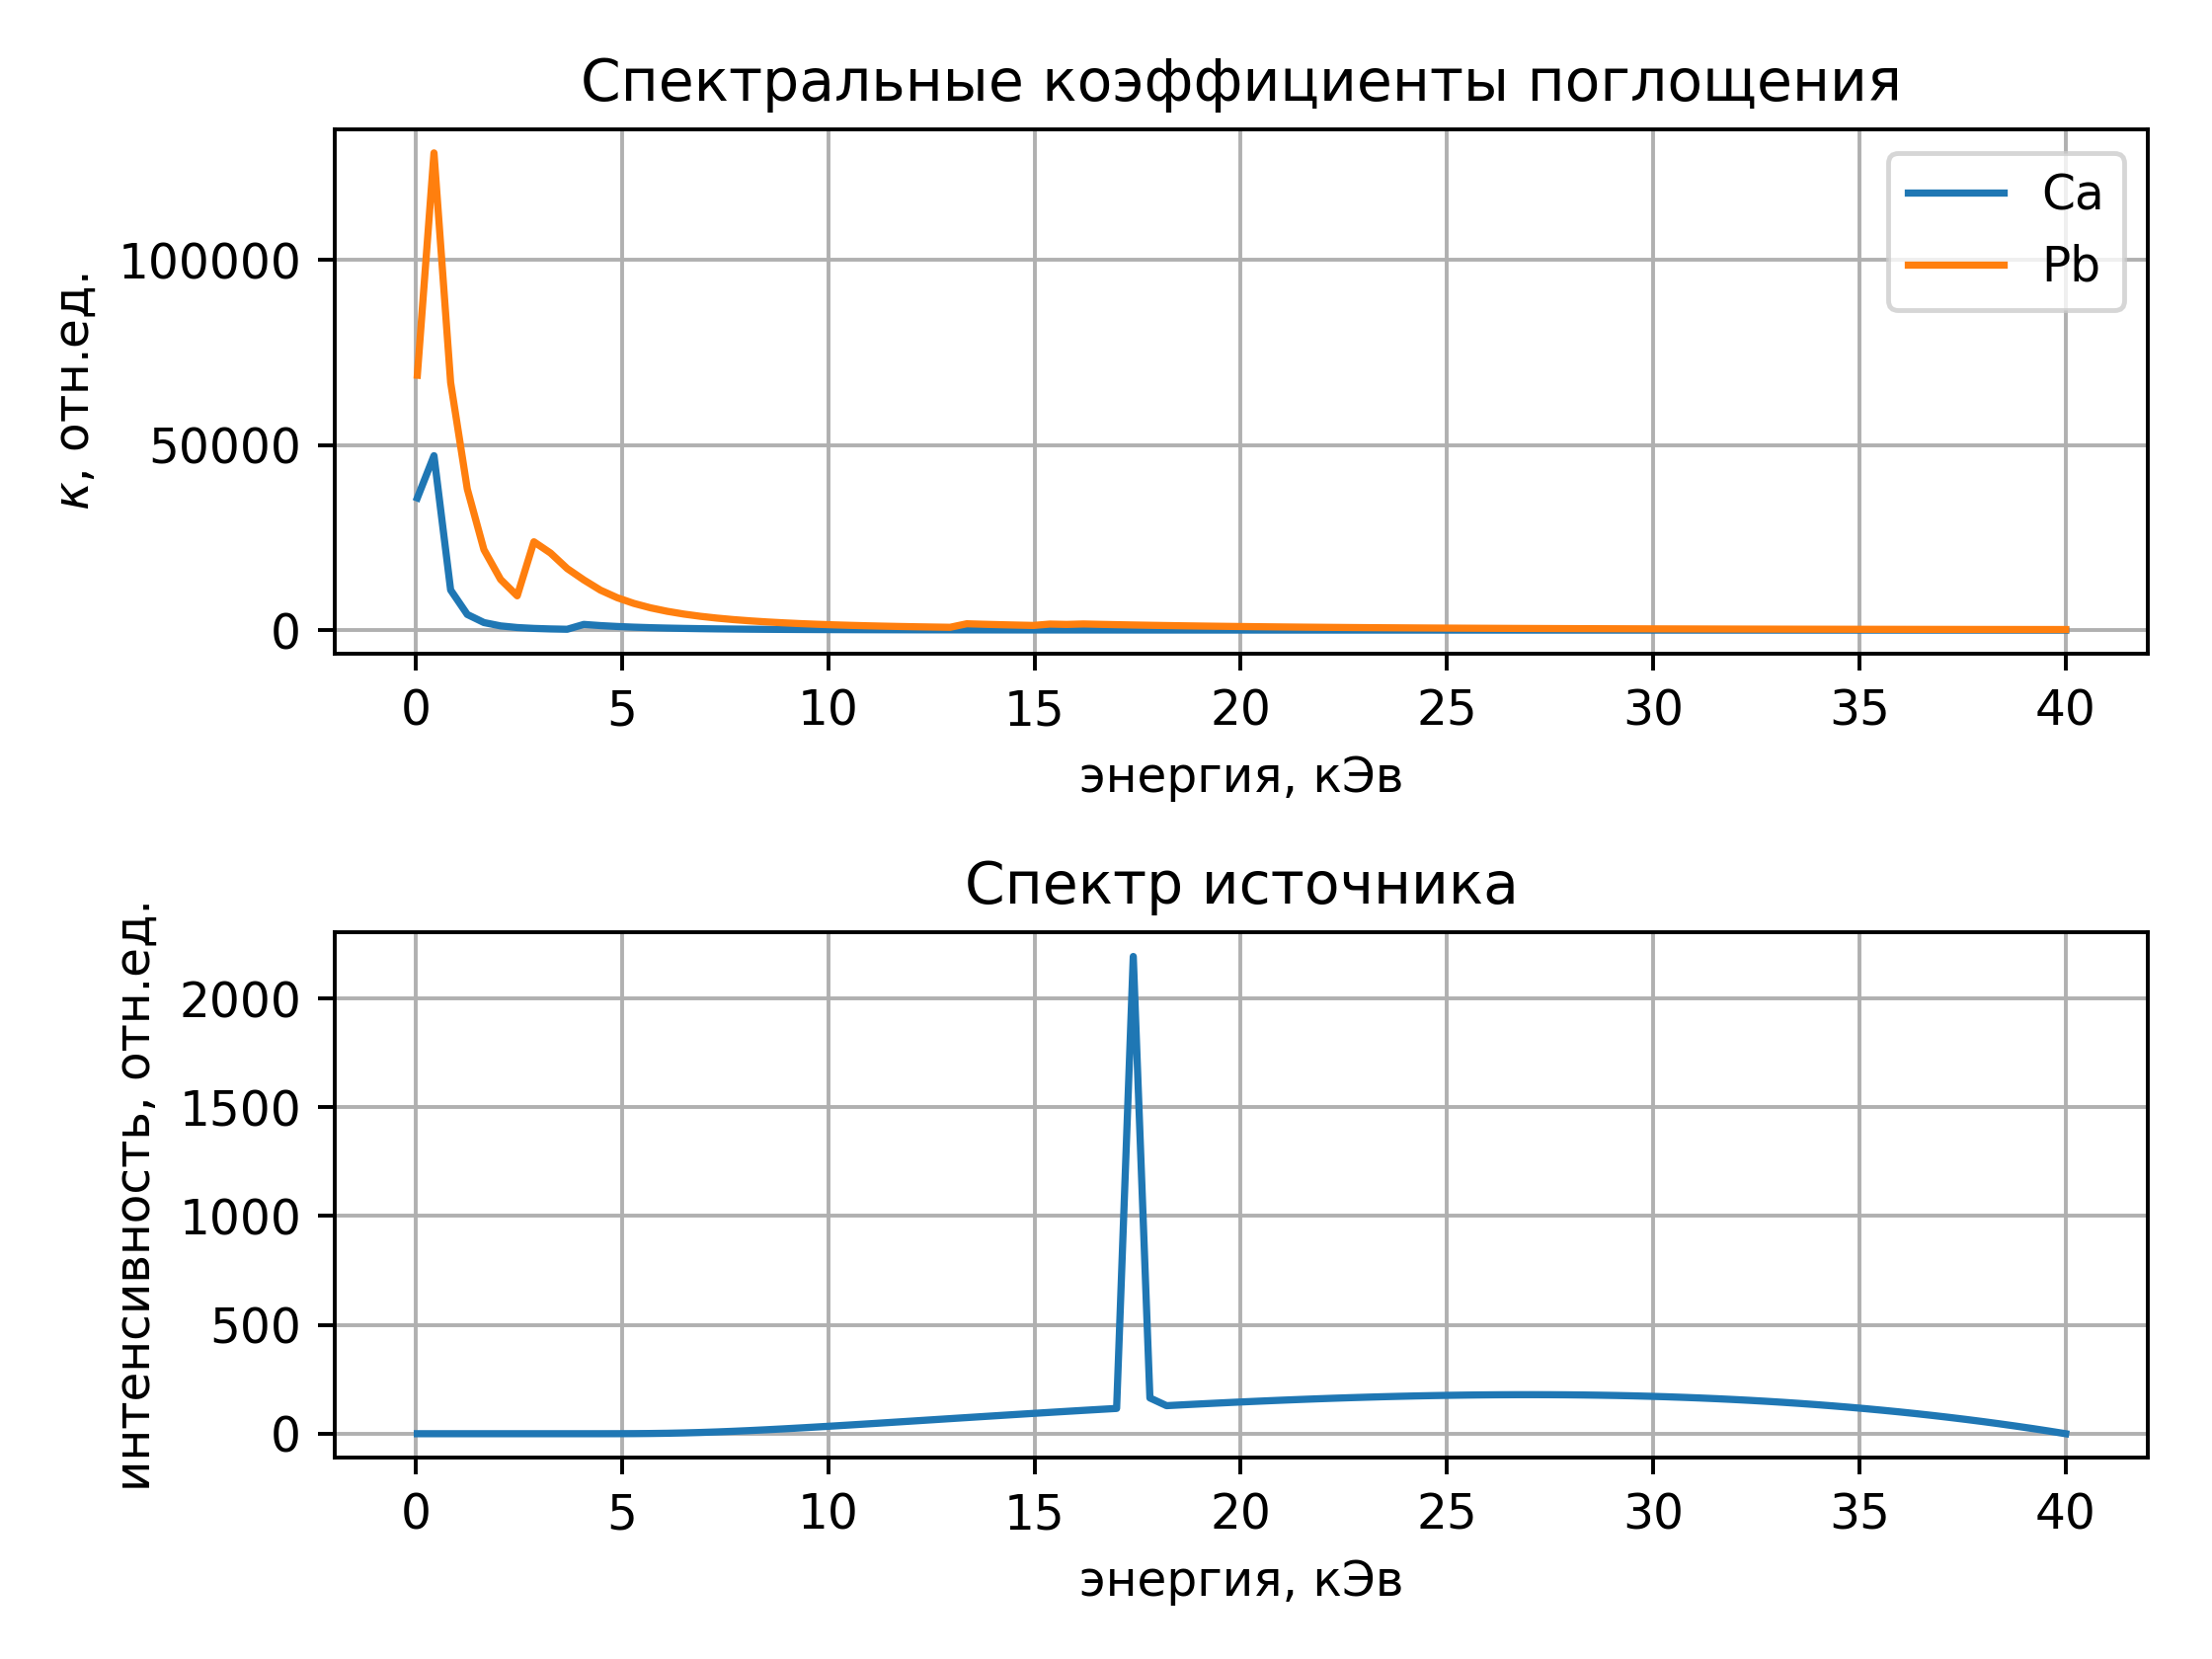
\includegraphics[width=1.1\textwidth]{zub_spectre}
\end{figure}
\end{column}
\end{columns}
\end{frame}

\begin{frame}
\frametitle{Реальные экспериметнальные данные}
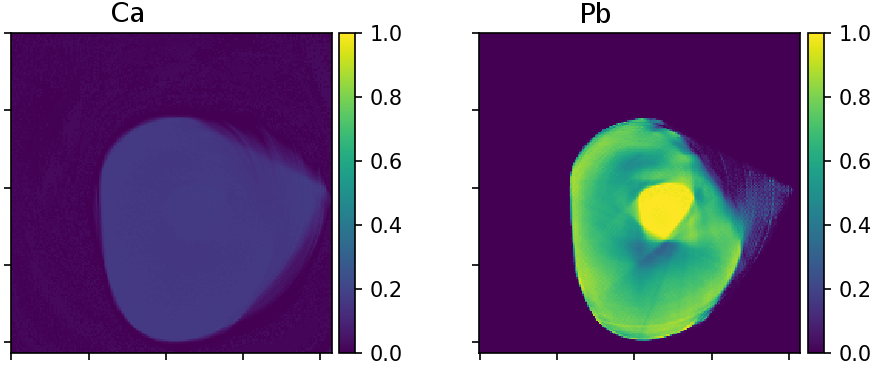
\includegraphics[width=\textwidth]{zub_wrm}
\end{frame}

\begin{frame}
\frametitle{Выводы}
\begin{itemize}
  \item Выведен шаг итерации в задаче, поставленной относительно концентраций
  \item Приведены результаты реконструкции на модельных и реальных экспериментальных данных
  \item Несмотря на то что методу не удается разделить концентрации, удается получить полезные свойства восстановленных картин
  \item Публикации \cite{cryst-2018, itas2015Prun}
\end{itemize}
\end{frame}


\begin{frame}
\begin{itemize}
  \item Рассмотрена задача восстановления в компьютерной томографии, основные подходы к ее решению.
  \item Построен асимптотически быстрый алгебраический метод FHT-SIRT, основанный на быстром преобразовании Хафа.
  \item Представлен метод восстановления, позволяющий уменьшить негативное влияние сильнопоглощающих включений в объекте.
  \item Предложен метод восстановления относительно концентраций различных элементов в объекте.
\end{itemize}
\end{frame}

\begin{frame}
\centering
%\vfill(5cm)
Спасибо за внимание!
\end{frame}

\begin{frame}
\frametitle{Приложение 1}
\framesubtitle{Полученные результаты}
\begin{itemize}
  \item Получен метод вычислительно эффективного вычисления транспонированного преобразования БПХ.
  \item Построен вычислительно эффективный алгебраический метод восстановления измерений компьютерной томографии на основе БПХ.
  \item Произведена адаптация метода для работы с данными реальных измерений. \item Произведено сравнение нового метода FHT-SIRT с традиционным SART
\end{itemize}
\end{frame}

\begin{frame}
\frametitle{Приложение 1}
\framesubtitle{Полученные результаты}
\begin{itemize}
  \item Построен метод восстановления рентгеновской томографии для объектов, содержащих сильнопоглощающие включения. 
  \item На реальных экспериментальных измерениях проведено исследование метода мягких ограничений, произведено сравнение с методом квадратичного программирования.
  \item Построен алгоритм восстановления томографии в задаче зондирования полихроматическим излучением. 
  \item Продемонстрированы результаты восстановления как синтетических, так и реальных экспериментальных данных
\end{itemize}
\end{frame}

\end{document} 

